\section{Output simplu}
\label{sec:output simplu}
La sfârşitul capitolului anterior, ai făcut cunoştinţă
cu primul tău cod PHP:
\lstinputlisting{cap01/info.php}

Prima linie marchează începutul procesării PHP. Ce se află
înaintea \texttt{<?php} este trimis aşa cum este către client.
Hai să testăm. Scrie ceva în tagul <h1> înainte de începutul
procesării PHP şi vezi ce iese:
\lstinputlisting{cap02/1-helloinfo.php}

PHP generează prea mult cod HTML pentru gusturile noastre simpliste, deci
fă cunoştinţă cu un cuvânt cheie în PHP: \texttt{echo}. Sintaxa
generală este:
\begin{verbatim}
echo <EXPR>;
\end{verbatim}
unde \texttt{EXPR}  trebuie să fie o expresie care evaluată, se reduce la o valoare.

\attention{Nu te speria dacă nu înţelegi totul, voi reveni asupra subiectului. Deocamdată urmează pur şi simplu paşii prezentaţi de mine, respectând sintaxa.
Simte-te liber să faci modificări, să experimentezi. Dacă faci ceva ce generează
o avertizare sau o eroare nu te impacienta, citeşte-o cu atenţie, încearcă
să o înţelegi, şi cere lămuriri pe wiki-ul proiectului.
}

Hai să-l învăţăm pe PHP să ne salute. În notepad++ crează un nou fişier
şi salvează-l ca \texttt{salut.php} în htdocs, apoi introdu codul:
\begin{lstlisting}
<?php
echo 'Salut Flavius';
\end{lstlisting}
Acum fă cu telnet o cerere HTTP, să vezi exact ce se întâmplă atunci când
interpreterul PHP execută acel cod:
\begin{verbatim}
GET /salut.php HTTP/1.1
Host: localhost
\end{verbatim}

Ce observăm? Exact! Observăm că nu vedem nici urmă de cod PHP, vedem doar
outputul generat de el. Nu tu \texttt{<?php}, nu tu \texttt{echo}. Asta
ne demonstrează că PHP ne-a procesat scriptul, script care a generat
output. Dacă scriptul nu ar fi generat output, \textit{response body}-ul
HTTP ar fi fost gol.

În al doilea rând, \textsl{http response body} nu conţine date în format HTML.
De ce? Simplu, deoarece nu i-ai spus niciunde să genereze nimic ce ar putea arăta a
HTML. Cum facem asta? O posibilitate ar fi următoarea:
\begin{lstlisting}
<?php
echo '<html><body>';
echo 'Salut Flavius';
echo '</body></html>';
\end{lstlisting}

Concluzia pe care o tragem este că PHP habar n-are ce este HTML. De ce?
După cum am spus atunci când ai instalat CLI-ul PHP (numit \texttt{php.exe}),
PHP este un limbaj de scripting general. De fapt nu este legat în niciun mod de
HTML sau de site-uri. Este doar felul în care îl folosim noi şi majoritatea
restului lumii. De fapt, PHP poate genera orice, imagini, documente, animaţii
(flash). Chiar nu eşti restrâns la HTML, dar nici nu te ajută în acest sens --
trebuie să scrii manual codul HTML, după cum ai văzut mai sus.

Vei vedea însă că îţi pune la dispoziţie constructe care înlesnesc generarea
de HTML -- de exemplu poţi genera o galerie de imagini aflate într-un anumit
director pe server, fără să trebuiască să ştii dinainte numele fişierelor.

Totuşi exemplul nostru anterior nu prea are sens -- nu este nimic dinamic în el.
L-am putea rescrie la fel de bine doar în HTML static, însă deoarece
vreau să demonstrez altceva, voi genera totuşi mesajul de salut cu PHP:
\begin{lstlisting}
<html>
	<body>
		<?php
		echo 'Salut Flavius';
		?>
	</body>
</html>
\end{lstlisting}

Observi că pentru a termina procesarea PHP şi a afişa din nou totul
aşa cum este (en. \textsl{unparsed}) se foloseşte \texttt{?>}.
În acest mod poţi porni şi opri procesarea PHP de oricâte ori doreşti în acelaşi fişier.
La sfârşitul fişierului procesarea este terminată automat, de aceea în exemplele
anterioare nu a fost nevoie de {\glqq}?>{\grqq}.

\attention{Mai observă şi cum mi-am făcut codul uşor de citit \textsl{indent}ându-l (en.
\textsl{to indent}), adică am aliniat deschiderea fiecărui tag HTML cu tag-ul
de închidere corespunzător, făcându-mi codul lizibil. Pentru codul nostru sursă
minuscul nu prea contează, însă diferenţa de mentenabilitate va fi
vizibilă când fişierele vor avea sute sau mii de linii de cod (LOCs en.
\textsl{lines of code}). Deci obişnuieşte-te
să indentezi codul apăsând tasta \keystroke{TAB} pentru fiecare nou nivel de
indentare necesar.}

Din acest punct înainte scopul nostru este să învăţăm PHP, nu să generăm
cod HTML valid, deci nu ne vom mai obosi să decorăm textul generat
cu \texttt{html} sau \texttt{body}. Însă nu uita că într-o pagină HTML
normală, validă, şi asta trebuie făcut, eventual
punând şi un
\textsl{doctype}\footnote{
\href{http://en.wikipedia.org/wiki/Document_Type_Declaration}{document type declaration}}, altfel
browserul intră în \href{http://en.wikipedia.org/wiki/Quirks_mode}{quirks mode}.

%----------------------------------------------------------
\section{Folosirea variabilelor}
Înainte de a trece la noţiuni noi, trebuie să revenim asupra exemplului nostru
cu câteva completări:
\begin{lstlisting}
<?php
echo 'Salut Flavius';
\end{lstlisting}
Ştim deja că \texttt{echo} este un cuvânt cheie care generează output pe baza
primului său parametru. Sper că ai intuit deja că fiecare instrucţiune
trebuie separată de următoarea prin ';'.

Însă ce este 'Salut Flavius'? Este o valoare în primul rând, pentru că
i-o putem pasa lui \texttt{echo}. În al doilea rând, este o constantă,
deoarece nu se modifică. La fiecare interpretare a scriptului, \textit{output}-ul
va fi acelaşi. Sumarizat: este o \textsl{valoare constantă}.

Pe lângă faptul că este o valoare constantă, mai este şi un \engl{şir de caractere}{string}.
Acesta este motivul pentru care
am pus mesajul între apostrofuri -- altfel PHP ar fi încercat să
interpreteze \textsl{Salut} şi \textsl{Flavius} ca constructe ale limbajului,
care evident nu există.

\good{Corect terminologic spunem deci că 'Salut Flavius' este un \textit{string constant} sau
mai pe larg \textit{o valoare constantă de tip string}.}

Deci încearcă! Fă-l pe PHP să genereze erori:
\begin{lstlisting}
<?php
echo Salut Flavius;
\end{lstlisting}
Mesajul de eroare ne-ar putea părea confuz:\\
\texttt{Parse error: syntax error, unexpected T\_STRING, expecting ',' or ';'}\\
Ceea ce se întâmplă este următorul lucru: PHP citeşte \texttt{echo}, şi deoarece a citit
şi a recunoscut instrucţiunea \texttt{echo}, intră în contextul semantic în care se aşteaptă ca următorul
lucru să fie o valoare, însă nu găseşte una, ci întâlneşte \texttt{Salut},
pe care nu-l recunoaşte\footnote{De fapt, parserul se blochează la {\glqq}Flavius{\grqq}, însă
ca să explic asta cum trebuie, ar fi trebuit să fi introdus deja constantele}
ca şi construct al limbajului.
De aceea ne spune că nu se aşteaptă să vadă T\_STRING-ul \texttt{Salut}.

Dar stai puţin, de ce îl numeşte {\glqq}T\_\textbf{STRING}{\grqq}, dar nu îl acceptă ca string?
Pentru a înţelege asta, trebuie să priveşti puţin lucrurile din perspectiva parserului
PHP. Codul sursă pe care îl scriem în limbajul PHP este folosit ca input pentru
parser. Acest input scris de noi este citit de PHP ca string, ca un şir de caractere.
Din acest motiv PHP ne spune foarte corect că nu se aşteaptă să vadă acel string acolo,
ci altceva.
\attention{Pentru PHP, codul scris de noi este un simplu text.}
Hai să vedem ce ar genera PHP dacă nu s-ar aştepta să vadă un string
din perspectiva noastră:
\begin{lstlisting}
<?php
echo 'Salut' 'Flavius';
\end{lstlisting}
ne zice \texttt{Parse error: syntax error, unexpected T\_CONSTANT\_ENCAPSED\_STRING}.

Ce înveţi din asta? În primul rând, înveţi că mesajele de eroare, deşi nedorite,
oferă informaţii preţioase despre ce s-a întâmplat. Din proprie experienţă
pot spune că vederea unui mesaj de eroare sau avertizare e ca o mână cerească,
reversul medaliei fiind mult mai frustrant: să nu vezi o eroare, dar codul
nici să nu funcţioneze aşa cum îţi imaginezi că ar trebui să funcţioneze -- sau
mai rău, să nu afişeze nimic, lăsându-te în întuneric complet. Deci fi fericit
când PHP îţi spune ce ai greşit, caută să înţelegi ce-ţi spune, şi apoi
repară-ţi greşeala.

Pe lângă stringuri, mai există şi alte tipuri de valori constante. PHP înţelege
\engl{numere întregi}{integers}, de exemplu \texttt{42},\footnote{Sunt curios
când va veni cineva să-mi spună de ce am ales 42 :-)}
numere cu virgulă (en, \textsl{floating point numbers} sau scurt \textsl{floats}),
unde partea zecimală
e separată de partea întreagă prin punct, de ex \texttt{3.1415}, şi alte lucruri
asupra cărora vom reveni. Hai să ne uităm la un exemplu:
\begin{lstlisting}
<?php
echo 'Salut 00';
echo 7;
echo '. PI este ~';
echo 3.1415;
\end{lstlisting}

\subsection{Variabile şi tipuri de date elementare}
Toate bune şi frumoase cu lucrurile cu care ai făcut cunoştinţă
până acum, însă ele nu te-au ajutat să creezi ceva dinamic.

Deci hai să facem un pas înapoi şi să ne gândim ce înseamnă şi
ce implică o eventuală dinamicitate. Pentru a fi dinamică, o
pagină trebuie să fie capabilă să primească date de intrare (\texttt{input}),
pentru a genera date de ieşire (\texttt{output}) pe baza acestora.

De exemplu, să zicem că vrem să facem o pagină care în loc să afişeze
mereu {\glqq}Salut Flavius{\grqq}, afişează {\glqq}Salut <nume>{\grqq}. Acest input (numele) trebuie
salvat undeva, altfel nu avem acces la el. Bine ai venit în lumea variabilelor.

O variabilă are trei caracteristici
\begin{enumerate}
\item un \textsl{nume} sau \textsl{identificator}
\item o \textsl{valoare} pe care o ţine
\item \textsl{tipul de date} (en. \textsl{datatype}) al valorii\footnote{mai
spunem colocvial şi \textit{tipul de date al variabilei} însă în PHP tipul
de date este inerent valorii -- vom reveni mai târziu asupra acestui aspect} precum
string, int sau float pe care le-ai cunoscut mai devreme
\end{enumerate}

Identificatorul variabilelor începe mereu cu \$, primul caracter după el
trebuie să fie o literă sau underscore (\_), iar următoarele
caractere pot fi litere, cifre, sau underscore.
Nu există o limită în lungimea identificatorului, şi nici restricţii privind
numirea lor. Există însă reguli nescrise pe care le vei întâlni mai târziu,
cât şi variabile pe care PHP le crează automat pentru tine.

Valoarea unei variabile poate fi orice bucată de informaţie ce poate
fi salvată.

Tipul de date al valorii poate fi unul din cele trei prezentate mai sus,
sau altele pe care le vom cunoaşte în acest capitol şi în capitolele următoare.

După cum am spus, \texttt{echo} afişează valoarea unei expresii.
Această valoare poate fi una constantă, precum în exemplele anterioare,
însă poate fi şi o variabilă. Exemplu:
\lstinputlisting{cap02/3-hello-var-error.php}
PHP ne va atenţiona cu o notificare că am încercat să accesăm o variabilă
nedefinită. Pentru a defini o variabilă trebuie să-i atribuim o valoare
mai întâi, iar asta o facem cu \textsl{operatorul} de atribuire \textsl{=}.
Putem spune şi că \textit{am salvat valoarea X în variabila Y}. Exemplu:
\lstinputlisting{cap02/4-hello-var.php}

\attention{\texttt{echo} nu adaugă automat spaţii niciunde. Este responsabilitatea
noastră să o facem. PHP chiar nu are noţiunea de {\glqq}cuvinte{\grqq}. Pentru el, un
şir de caractere este un şir de caractere şi atât.} 

În cazul de faţă, variabila \texttt{\$nume} nu prea îşi are rostul, deoarece o
folosim o singură dată. Însă imaginează-ţi că ai un script lung,
şi vrei să refoloseşti acel nume în diferite locuri în cadrul generării de
output. Variabilele sunt ideale pentru acest lucru, deoarece nu trebuie
decât să schimbi valoarea într-un loc, iar schimbarea va fi preluată în
întregul script:
\lstinputlisting{cap02/5-hello-var-reuse.php}

Felicitări, ai creat primul tău script care reutilizează variabile.

\subsection{Operaţii cu string, int, float}
Cu aceste tipuri de date se pot face operaţii. În primul rând,
stringurile pot fi \textsl{concatenate}, indiferent dacă sunt salvate
în variabile sau provin din valori constante. A concatena
înseamnă a lipi un string de următorul, pentru a forma un nou string.
Exemple:
\lstinputlisting{cap02/6-concatenare-stringuri.php}

\textit{Linia 2} face următorul lucru: mai întâi concatenează cele două valori constante
'Salut ' şi 'Flavius', operaţie în urma căreia rezultă \textsl{valoarea intermediară}
'Salut Flavius'. Îţi poţi imagina că această valoare stă acum de partea
dreaptă a operatorului de atribuire. Iar deoarece avem o atribuire, această
valoare intermediară este salvată în variabila \texttt{\$a}.

\textit{Linia 3} afişează valoarea salvată în variabila \texttt{\$a}.

Ne-am fi putut folosi de acea {\glqq}valoare intermediară{\grqq} de pe linia 2 afişand-o direct:
\begin{lstlisting}
<?php
echo 'Salut ' . 'Flavius';
\end{lstlisting}
Aici valoarea intermediară \textit{care rezultă în urma concatenării} celor două stringuri
constante este pasată direct (ca o nouă valoare) instrucţiunii \texttt{echo}.

După cum ai observat pe \textit{linia 2}, operaţia de atribuire este interpretată
de PHP de la dreapta la stânga. Mai întâi sunt făcute rând pe rând operaţiile
din partea dreaptă a atribuirii, apoi valoarea rezultată este salvată în
variabila aflată în stânga atribuirii. Datorită acestei ordini spunem că
operaţia de \engl{atribuire}{assignment} este \textsl{right-associative}.

\textit{Linia 5}: Datorită asociativităţii de dreapta a operaţiei de atribuire,
într-o atribuire putem folosi o variabilă precum \texttt{\$a} în partea dreaptă, genera
o valoare temporară pe care o atribuim tot variabilei \texttt{\$a}, suprascriind
valoarea sa iniţială. Dacă am fi ştiut că mai avem nevoie de nume ca valoare
de sine stătătoare, pe linia 5 ar fi trebuit să introducem o nouă variabilă
căreia să-i atribuim noua valoare,
astfel încât să nu pierdem valoarea iniţială a lui \texttt{\$a}.
Însă în cazul nostru, \textit{linia 5} este extrem de curată,
deoarece nu introduce o nouă variabilă în mod inutil.

Să revenim la sintaxă şi la semantică. Sintaxa lui echo este:\\
\texttt{echo <EXPR>;}\\
Iar a operaţiei de concatenare este:\\
\texttt{<expr1> . <expr2>}\\
<expr1> şi <expr2> pot fi orice fel de expresii, fie ele valori constante,
sau variabile -- deoarece variabilele au şi ele o valoare pe care
o cară cu ele. În urma operaţiei de concatenare rezultă o valoare
intermediară. Chiar dacă aceasta e {\glqq}invizibilă{\grqq} (deoarece
PHP o crează în mod transparent pentru noi), ea este tot o valoare ca oricare
alta, deci poate fi pusă oriunde PHP ne lasă să punem o expresie.

Dar stai puţin, operaţia de concatenare însăşi acceptă două expresii!
Consecinţa? Putem concatena acele valori intermediare, transparente,
într-un lanţ\footnote{În matematică spunem că abordăm problema
\href{http://en.wikipedia.org/wiki/Structural_induction}{inductiv}.}:\\
\texttt{<valoare1> . <valoare2> . <valoare3> . <valoareN>}

În astfel de cazuri, <valoare1> este concatenată cu <valoare2> şi rezultă
o valoare intermediară, transparentă, care este apoi concatenată cu <valoare3>,
şi tot aşa.
Exemplu:
\lstinputlisting{cap02/7-concatenare-stringuri.php}

Despre limbajul PHP se spune că este \textsl{dynamically typed}. Asta înseamnă
că poate (în limitele {\glqq}bunului simţ{\grqq}), să convertească automat
o valoare de un tip, într-o altă valoare de alt tip, care e cât
mai apropiată de valorea iniţială. Aşa se face că deşi operatorul
de concatenare acceptă doar doi parametri de tip string, putem totuşi
concatena şi numere. PHP va crea însă încă o valoare intermediară
cu reprezentarea valorii iniţiale ca string. Un exemplu:
\lstinputlisting{cap02/8-concatenare-inference.php}

\attention{Încearcă să eviţi a-l forţa pe PHP să
trebuiască să convertească un număr într-un string,
deoarece operaţia asta consumă resurse inutil.
În schimb foloseşte sintaxa alternativă a lui \texttt{echo}
cu care vei face cunoştinţă în continuare.}

\begin{Exercise}[title={Primul cod propriu}]
Continuă codul următor astfel încât să afişeze\\
\texttt{Valoarea lui PI este 3.1415.}
\lstinputlisting{cap02/9-ex-pi.php}
\end{Exercise}

Există o sintaxă alternativă pentru \texttt{echo}, care ne permite
să afişăm valori constante amestecate cu valori variabile fără
a mai crea valori intermediare, deci PHP poate executa
scriptul mai rapid şi cu consum mai mic de memorie.
Pentru asta punem virgulă între valori:
\lstinputlisting{cap02/10-echo-list.php}

Asta înseamnă practic că \texttt{echo} va fi apelat asupra fiecărui
parametru din listă. Atenţie: diferenţele se pot vedea
doar atunci când lucrezi cu cantităţi mari de informaţie.

\begin{Exercise}[difficulty=1,title={Sintaxa alternativă pentru echo}]
De câte ori va fi apelat \texttt{echo} în codul următor? % de 3 ori
\begin{lstlisting}
<?php
echo 'Salut ', 'Homer ' . 'Simpson.' , ' Ce ' . 'faci?';
\end{lstlisting}
\Question o dată
\Question de trei ori
\Question de cinci ori
\end{Exercise}

\begin{Exercise}[difficulty=2,title={Determinarea fluxului de execuţie într-un exemplu simplu}]
Explică cum crezi că execută PHP următoarea linie, cât mai concret posibil, aşa cum
ai văzut în explicaţiile anterioare.
\lstinputlisting[label=lst:execflow echo,caption={echo'ing an assignment}]{cap02/12-ex-execflow.php}
\end{Exercise}

\subsection{Operaţii matematice}

PHP ştie toate cele patru operaţii aritmetice: + pentru adunare,
- scădere, * înmulţire şi / pentru împărţire. Ştie şi că
înmulţirea şi împărţirea sunt de gradul doi, iar dacă ai nevoie
de altă ordine a operaţiilor poţi folosi paranteze rotunde pentru
grupare. Parantezele crează deasemenea valori intermediare, ca
şi operatorul de concatenare.

Rezultatele pot fi atribuite variabilelor, deoarece sunt tot
valori, pot fi afişate, sau chiar concatenate. Nu trebuie decât
să pui cap la cap ce ai învăţat până acum şi să-ţi laşi imaginaţia
să zboare.
Un exemplu cu operaţii matematice de la simple la complexe:
\lstinputlisting[caption=Operaţii matematice,label=lst:math opers]{cap02/11-math-opers.php}

Majoritatea lucrurilor ar trebui să-ţi fie cunoscute. Liniile
2-11, 19 şi 24 conţin aşa-numite comentarii. Există două
tipuri de comentarii, cele care se întind pe mai multe linii
şi încep cu {\glqq}/*{\grqq} şi se termină cu {\glqq}*/{\grqq}. Al doilea tip
începe cu {\glqq}//{\grqq} şi se termină la sfârşitul liniei.

Menirea unui comentariu este să documenteze sau să marcheze
anumite lucruri în cod. Când scripturile tale vor deveni foarte complexe,
vei vrea să le documentezi comentându-le, astfel încât să-ţi
poţi aminti uşor ce face codul şi de ce o face.

\attention{Comentariile sunt ignorate de PHP. Ele conţin
practic metadate despre codul însuşi, utile doar programatorului.}
\good{Încearcă să nu pui comentarii stupide, precum:
\lstinputlisting{cap02/13-useless-comment.php}
Lasă codul să vorbească de la sine, pe cât posibil. Documentează
variabilele introduse şi felul în care sunt folosite. Documentează
algoritmii complecşi. Încearcă să-ţi imaginezi ce nu ar înţelege
din prima cineva care ţi-ar vedea codul pentru prima oară şi
documentează acele lucruri.}
\attention{
Asteriscurile de pe
liniile 3-10 nu sunt necesare, însă este un standard
mai mult sau mai puţin nescris să îţi formatezi în acest fel
comentariile care documentează codul. Standardul
vine din lumea java, unde acestea se numesc
\textsl{javadocs}\footnote{
Javadoc
}. Şi în PHP, ca şi în java, există scule care extrag informaţiile
din \textsl{docblocks} şi generează automat documentaţie.

%TODO CHAP exact care capitol? pune 6 cand e gata cartea
În capitolele următoare vei face cunoştinţă cu
astfel de scule. Deocamdată obişnuieşte-te să
îţi documentezi codul cum trebuie, chiar dacă
scripturile scrise de tine sunt mici şi nu simţi
nevoia de a le documenta. Scrierea documentaţiei
te ajută să îţi fixezi mai bine lucrurile învăţate.
}
\footnotetext{\url{http://en.wikipedia.org/wiki/Javadoc}}

Comentariile mai pot fi folosite de programator
şi ca un mijloc rapid de a testa diferite funcţionalităţi.
Să zicem că ai două soluţii posibile pentru rezolvarea
unei anumite probleme. O poţi comenta pe prima, şi
o lăsa doar pe a doua să fie executată. De exemplu:

\begin{lstlisting}
<?php
//echo 1+4*3;
echo (1+4)*3;//calculeaza corect, cu paranteze
\end{lstlisting}

Pentru a reprezenta numere negative, întregi (int)
sau cu virgulă (float), nu trebuie decât să pui un
minus în faţa lor. De exemplu:

\begin{lstlisting}
<?php
echo -4 + -3;
\end{lstlisting}

Deseori vei fi în situaţia de a vrea
să faci o operaţie matematică
asupra valorii unei variabile,
şi să salvezi rezultatul în aceeaşi variabilă.
Pentru astfel de cazuri, poţi combina operatorii
matematici +,-,*,/ cu operatorul de atribuire. Câteva
exemple:
\begin{lstlisting}
<?php
$a = 7;
echo 'a este ',$a,'<br>';
$a += 2;//sau pe lung $a = $a + 2;
echo 'a += 2 face ',$a,'<br>';
$a /= -3;// $a = $a / 3;
echo 'a /= -3 este ',$a,'<br>';
\end{lstlisting}

De fapt, poţi combina chiar şi operatorul de concatenare
cu atribuirea:
\begin{lstlisting}
<?php
$a = 'Hello';
$a .= ' world';
\end{lstlisting}

\begin{Exercise}[title={Lipsă output}]
De ce codul următor nu afişează nimic?
\begin{lstlisting}
<?php
$a = 'Hello';
$a .= ' world';
\end{lstlisting}
\end{Exercise}

\label{term:modulo}
Mai există încă un operator matematic foarte interesant numit \textsl{modulo},
cu simbolul \texttt{\%}. Operaţia modulo are ca rezultat restul
împărţirii primului \textsl{operand} la al doilea. Exemplu:
\begin{lstlisting}
<?php
echo 11 % 3;
\end{lstlisting}
Este interesant deoarece cu el putem determina dacă un număr este multiplul
unui alt număr.


Liniile 20-22 din exemplul \ref{lst:math opers}
introduc variabile intermediare noi în care
salvăm valorile unor calcule. Asta nu este neapărat greşit,
însă noi variabile trebuie introduse doar atunci când
ştii că vei avea de gând să refoloseşti (de cel puţin
două ori) o valoare, sau când o valoare trebuie să
se schimbe de-a lungul execuţiei scriptului, dinamic
(căci asta spune însuşi termenul de \textit{variabilă}).
De exemplu, să zicem că vrei să saluţi vizitatorul
cu {\glqq}Bună dimineaţa{\grqq}, {\glqq}Bună ziua{\grqq} sau {\glqq}Bună seara{\grqq}
în funcţie de ora actuală a Bucureştiului.

Deoarece noi folosim acele variabile intermediare
\texttt{\$c\_area}, \texttt{\$r\_area} şi \texttt{\$r\_perim} o singură dată, am
putea renunţa la ele şi am putea pasa rezultatele
calculelor direct lui \texttt{echo},
fără a le mai salva în variabile. Astfel, linia 25
ar deveni:
\lstinputlisting{cap02/14-math-in-echo.php}

\good{Inventează variabile noi doar atunci când ai
nevoie de ele. Variabilele ocupă memorie
de lucru şi mănâncă timp la procesare. 
}
\attention{
În plus, în unele cazuri, prea multe variabile
îţi pot face scriptul greu de înţeles. Însă acest
lucru este valabil şi dacă introduci prea puţine
variabile. Sfatul anterior rămâne valabil şi
în acest caz: gândeşte-te bine când şi \textit{dacă}
ai nevoie de o nouă variabilă, şi introdu
una nouă în mod \textit{responsabil}.
}

\begin{Exercise}[difficulty=1,title={Primul pas spre creativitate}]
\ExePart
Uită-te încă o dată pe exemplul \ref{lst:math opers} cu atenţie,
încearcă să-ţi impregnezi sintaxa şi outputul, apoi închide
cartea, scoate un \textit{creion} şi o \textit{foaie de hârtie}
şi scrie un cod similar care să facă acelaşi lucru.

Poate fi un cod \textit{complet diferit}, nu trebuie să fie acelaşi,
şi nici variabilele nu trebuie numite la fel. Funcţionalitatea
trebuie însă să fie \textit{asemănătoare}!

\textit{Apoi} transcrie codul de pe foaie într-un fişier
PHP şi rulează-l. 99\% din începători vor face greşeli,
ceea ce e bine. Doar aşa ţi se vor impregna în minte anumite lucruri.

\attention{Programarea pe hârtie este cea mai sănătoasă, mai ales
pentru un începător. Te provoc să îmi urmezi sfatul, pentru
că îl dau din proprie experienţă.}
\ExePart
Completează scriptul astfel încât să afişeze şi volumul cubului
de latură \texttt{\$a}.
\end{Exercise}



\section{Algoritmi şi scheme logice}
Un algoritm este un set de instrucţiuni bine definit
care descrie pas cu pas ce trebuie făcut pentru
a rezolva o problemă dată.

Atunci când scriem un cod PHP, textul pe care
îl scriem în întregimea sa este descrierea unui algoritm.

Cum calculatoarele actuale sunt simple maşini şi nu
dispun de inteligenţă, algoritmii pe care îi concepem
trebuie să fie foarte exacţi, lipsiţi de ambiguităţi.

Îţi poţi imagina că până acum PHP executa instrucţiune
cu instrucţiune scripturile noastre, fiecare instrucţiune
fiind separată de următoarea prin ';'.
Deoarece PHP executa toate instrucţiunile exact în ordinea
în care le citea, spunem că până acum execuţia a fost
\textit{liniară}.

Limbajul PHP ne pune la dispoziţie constructe pentru a bifurca
execuţia. Îţi poţi imagina că, atunci când PHP
execută un cod, se plimbă cu un fel de cursor
pe deasupra {\glqq}textului{\grqq}. Folosind o astfel de bifurcaţie
i-am putea spune "dacă o condiţie C este adevărată, fă
X, dacă nu (altfel) fă Y" sau la fel de bine
i-am putea spune "atâta timp cât condiţia C
este adevărată, fă X".

Descrierile în cuvinte de mai sus {\glqq}dacă ... atunci ...{\grqq}
sau {\glqq}atâta timp cât ...{\grqq} pot fi formalizate în ceea
ce numim \textsl{limbaj pseudocod}. 

Limbajul pseudocod ne permite să descriem algoritmi
folosind limba română, aşa cum am folosit metalimbajul
din secţiunea trecută pentru a descrie sintaxa limbajului HTML.

Pseudocodul nu are o sintaxă strictă, însă e bine să
ne exprimăm cât mai clar şi punctual, fără omisiuni.

De exemplu, un algoritm de autentificare ar putea
fi specificat astfel:
\begin{lstlisting}[language=pseudocod]
daca parola este corecta
	afiseaza 'autentificat'
altfel
	afiseaza 'acces restrictionat'
\end{lstlisting}
%\begin{Verbatim}[commandchars=\\\{\}]
%\nl{1}\textbf{dacă} parola este corectă
%\nl{2}	afişează 'autentificat';
%\nl{3}\textbf{altfel}
%\nl{4}	afişează 'parola greşită';
%\end{Verbatim}
Însă acesta este incomplet! De unde vine
acea {\glqq}parolă{\grqq} pe care am menţionat-o pe linia 1?

Calculatoarele sunt stupide, şi la fel este şi PHP. Va
trebui să-i spunem mai întâi că citim acea parolă:
\begin{lstlisting}[language=pseudocod]
citeste parola
daca parola este corecta
	afiseaza 'autentificat'
altfel
	afiseaza 'acces restrictionat'
\end{lstlisting}

Sună stupid, probabil ar trebui să ne aşteptăm
ca electronica din CPU să ghicească cumva
ce vrem de la ea. Deocamdată asta nu este posibil,
în mare parte deoarece dispozitivele electronice,
inclusiv un
CPU,\footnote{\href{http://en.wikipedia.org/wiki/Central_processing_unit}{Central Processing Unit}} nu sunt inteligente.
Până când nu va apărea inteligenţa artificială,
va trebui să ne resemnăm cu faptul că e responsabilitatea
noastră de fiinţe inteligente să gândim şi să
concepem algoritmi pentru maşini, pe care
acestea să le urmeze pas cu pas.

Pe linia 2 a algoritmului anterior are loc o bifurcaţie.
La rulare, PHP ar decide dacă {\glqq}parola este corectă{\grqq}, şi dacă
da, va trece cu cursorul său {\glqq}de execuţie{\grqq} prin \textit{linia 3},
altfel va trece prin \textit{linia 5}. 

Te rog fi atent cum indent-area codului reflectă cărei {\glqq}cărări{\grqq}
din această bifurcaţie aparţine fiecare din cele două instrucţiuni
{\glqq}afişează{\grqq}.

Să zicem că vrem să afişăm {\glqq}Salut <autentificat|necunoscut>. Ce faci?{\grqq},
unde algoritmul decide pe baza unui input {\glqq}parolă{\grqq} ce să afişeze, {\glqq}autentificat{\grqq}
sau {\glqq}necunoscut{\grqq}, însă în ambele cazuri să fie afişat {\glqq}Salut {\grqq} şi {\glqq}. Ce faci?{\grqq}.

Un astfel de algoritm ar putea arăta astfel:
\begin{lstlisting}[language=pseudocod]
citeste parola
afiseaza 'Salut '
daca parola este corecta
	afiseaza 'autentificat'
altfel
	afiseaza 'necunoscut'
afiseaza '. Ce faci?'
\end{lstlisting}

Liniile 1 şi 2 vor fi executate liniar, iar la linia 3 bifurcăm \textsl{fluxul de execuţie}.
Dacă parola citită este corectă, fluxul de execuţie va trece prin linia 4, altfel
el va trece prin linia 6. Linia 7 însă nu se află într-o bifurcaţie, ci continuă
execuţia liniară din care fac parte şi liniile 1 şi 2 şi de fapt şi 3.

Exact, şi linia 3 face parte din execuţia liniară, deoarece acea verificare "este
parola corectă?" va fi executată de fiecare dată.

\begin{Exercise}[title={Execuţia liniară conţine şi verificarea condiţiei},difficulty=1]
De ce face parte şi verificarea unei condiţii din execuţia liniară de dinainte şi de după
{\glqq}dacă{\grqq}?
\end{Exercise}


Fluxul de execuţie este constituit din {\glqq}locurile{\grqq} prin care plimbăm
acel {\glqq}cursor{\grqq} folosit de PHP pentru a executa fiecare instrucţiune.
Acest flux este dinamic, se poate schimba la rularea scriptului,
folosind exact aceste constructe ale limbajului precum {\glqq}dacă{\grqq} sau {\glqq}atâta timp cât{\grqq},
constructe pe care le vom cunoaşte în paginile viitoare.

Aşa cum putem descrie un algoritm folosindu-ne doar de text, putem
descrie un algoritm şi prin scheme grafice. Aceste scheme grafice se numesc
\textit{scheme logice} (en. \textsl{flowcharts}).

Figura \ref{fig:flowchart authenticated} este transpunerea
într-o schemă logică a algoritmului descris în pseudocodul anterior.

\begin{figure}[h!]
  \centering
    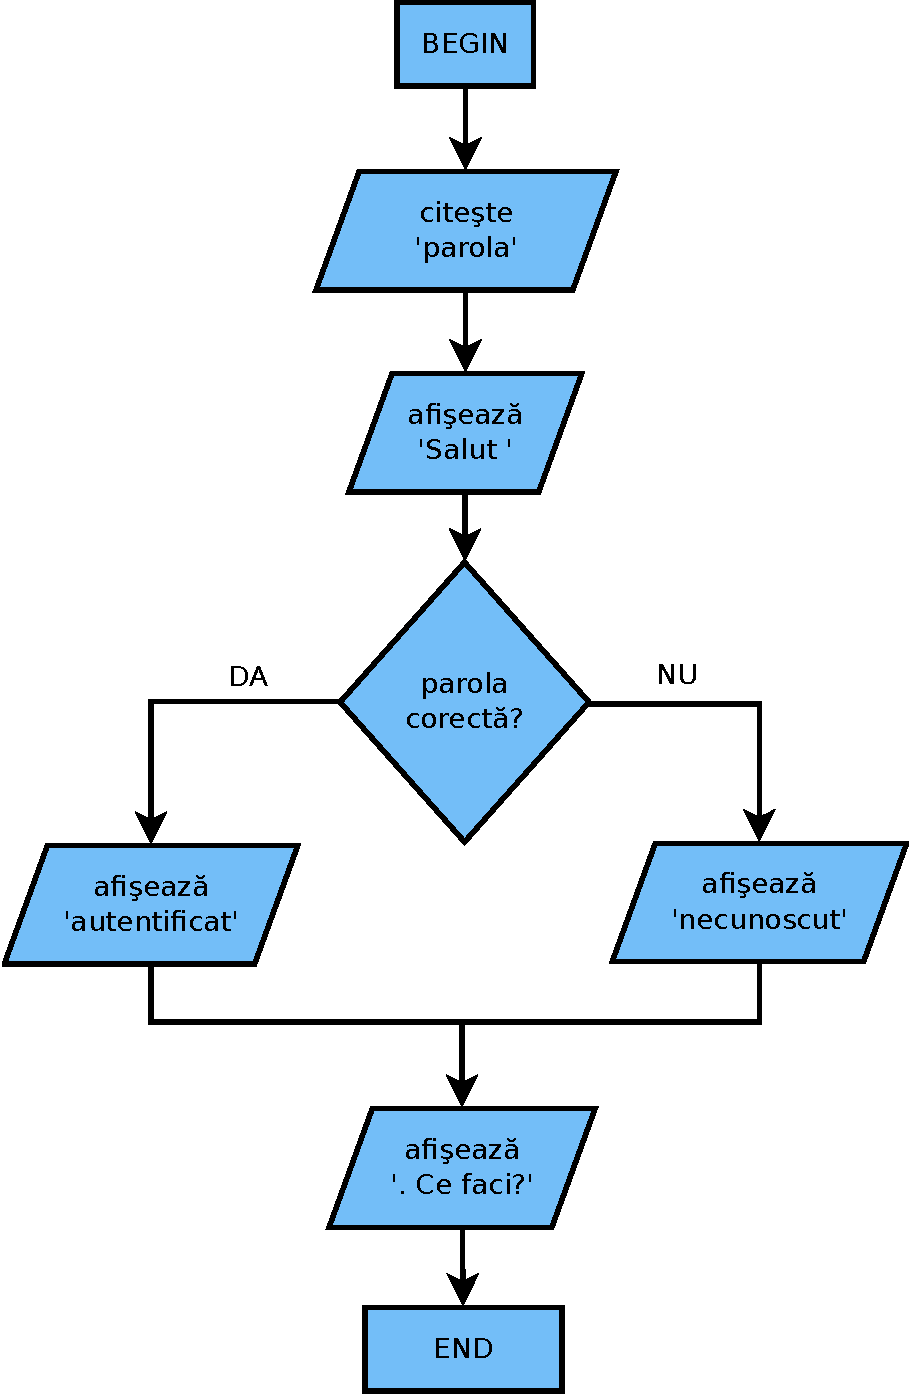
\includegraphics[scale=.5]{cap02/flowchart1-crop.pdf}
  \caption{Flowchart autentificare}
  \label{fig:flowchart authenticated}
\end{figure}

%\needspace{4\baselineskip}
Regula de bază la interpretarea unei scheme logice
este să urmezi în mod stupid săgeţile, la fel ca şi
coiotul nostru din figura \ref{fig:coyote arrow}.

O schemă logică are doar un singur bloc {\glqq}BEGIN{\grqq}, şi unul
sau mai multe blocuri {\glqq}END{\grqq}. O schemă logică curată
ar trebui să aibă totuşi un singur bloc {\glqq}END{\grqq}
către care conduc toate {\glqq}cărările{\grqq} de execuţie posibile.

Operaţiile de input/output sunt puse în paralelograme,
iar operaţiile decizionale sunt puse în romburi şi au
una sau două ieşiri, pentru cazurile {\glqq}DA{\grqq} respectiv {\glqq}NU{\grqq}
în care condiţia este adevărată sau falsă.

\begin{figure}[h!]
  \centering
    
\includegraphics[scale=.8]{cap02/coyote-arrow.png}
  \caption{Cum să urmezi săgeţile}
  \label{fig:coyote arrow}
\end{figure}

Revenim asupra definiţiei fluxului de execuţie, folosindu-ne de scheme logice de data asta:
\textit{fluxul de execuţie} este constituit din săgeţile concrete parcurse de PHP
la executarea scriptului.

\begin{Exercise}[difficulty=2,title={Găseşte eroarea de logică}]
\ExePart
Care sunt greşelile algoritmice din pseudocodul următor?

\begin{lstlisting}[language=pseudocod]
daca parola este corecta
	afiseaza 'autentificat'
altfel
	afiseaza 'parola este gresita'
afiseaza 'aceasta este o informatie secreta '
afiseaza 'vizibila doar utilizatorilor autentificati'
\end{lstlisting}

Identifică-le, explică-le în cuvinte, şi rescrie pseudocodul corect.

Foloseşte-ţi intuiţia pentru a determina ce ar trebui
să facă un astfel de algoritm şi ce nu, pe baza outputului.

\ExePart
Desenează două scheme logice, una pentru pseudocodul (greşit)
din partea I a exerciţiului, şi una pentru varianta corectă
a pseudocodului pe care ai găsit-o ca soluţie în partea I.
\end{Exercise}


\section{Tipul de date boolean. Expresii logice}
\label{sec:tipul de date boolean. Expresii logice}

Secţiunea anterioară a tratat {\glqq}parola este corectă{\grqq} ca ceva
de la sine înţeles. Poate pentru noi este uşor de înţeles,
însă PHP, şi algoritmii în general, nu au noţiunea de {\glqq}corect{\grqq}.

Ce înseamnă {\glqq}corect{\grqq} de fapt? Cum determinăm noi, oamenii,
dacă o adresă, un nume, sau în cazul de faţă o parolă, este corectă?
Ceea ce facem este de fapt compararea a ceva ce vine din exterior, a
unui input, cu ceea ce considerăm noi {\glqq}corect{\grqq}, pe baza cunoştinţelor
sau experienţelor {\glqq}salvate{\grqq} în creierul nostru.\footnote{Procesele
cognitive sunt omise în mod conştient, pentru a simplifica imaginea.}

De exact acest lucru are nevoie şi PHP. Bine ai venit în lumea
expresiilor logice. 

Există nenumăraţi operatori logici. Însă înainte de a trece
la ei, trebuie să introducem o funcţie numită \texttt{var\_dump()}.
În capitolul următor vei învăţa despre funcţii pe larg,
însă deocamdată o mică definiţie: \textit{O funcţie este
ca o {\glqq}cutie neagră{\grqq}. O hrăneşti cu parametri, şi ea face ceva cu
acele valori}. În cazul nostru, vom folosi funcţia \texttt{var\_dump()}
în loc de cuvântul cheie \texttt{echo} pentru a afişa atât valoarea
pe care i-o pasăm ca parametru, cât şi tipul său de date. \texttt{echo}
nu ar fi bun pentru asta deoarece ar face automat nişte conversii
între tipuri de date, şi exact acele tipuri de date sunt ceea ce
vrem să vedem neschimbat.


Toate expresiile logice, care conţin operatori
logici,\footnote{nu neapărat, dar voi vorbi mai târziu
despre asta} sunt evaluate şi au în final
fie valoarea {\glqq}adevărat{\grqq}, fie valoarea {\glqq}fals{\grqq}. Deoarece
expresiile logice sunt atât de importante,\footnote{Există
chiar şi o matematică care le susţine.}
pentru ele există şi un tip de date: \textsl{boolean}, sau pe scurt: bool.
Acesta este al patrulea tip de date cu care faci cunoştinţă, după
string (şir de caractere), int (integer -- număr întreg)
şi float (număr cu virgulă).

În contrast cu celelalte tipuri de date, informaţii de tipul
boolean nu pot avea decât două valori: \texttt{TRUE} sau \texttt{FALSE}.

De exemplu, într-o aplicaţie complexă, în care unii utilizatori
au drepturi speciale, am putea întâlni:
\begin{lstlisting}
$este_administrator = TRUE;
\end{lstlisting}
Însă în loc de \texttt{echo}, vom folosi \texttt{var\_dump()}, în felul următor:
\begin{lstlisting}[firstnumber=2]
var_dump($este_administrator);
\end{lstlisting}
Încearcă, să vezi ce îţi afişează. Bineînţeles că poţi afişa şi valorile
constante \texttt{TRUE} sau \texttt{FALSE} direct:
\begin{lstlisting}
<?php
var_dump(TRUE);
var_dump(FALSE);
\end{lstlisting}

Acum că ştim cum se foloseşte o funcţie precum \texttt{var\_dump()},
hai să revenim la ideea noastră iniţială: PHP nu ştie ce
înseamnă pentru noi {\glqq}parolă corectă{\grqq}, deci trebuie să confruntăm
cele două valori şi să decidem dacă ele sunt una şi aceeaşi.

Aici intră operatorul de comparaţie în joc, \texttt{==}. Acesta
este capabil să compare valorile a două expresii.

\attention{Din lucrul nostru cu \texttt{echo} din secţiunile anterioare,
ştii că o expresie poate fi orice are o valoare, fie ea constantă,
variabilă, rezultatul unei concatenări sau de ce nu, rezultatul
unor operaţii matematice.}

Ne putem da seama cu uşurinţă cum funcţionează următorul cod:
\begin{lstlisting}
<?php
$input = 'asdfgh';//conform unor studii, o parola foarte des folosita

echo '3==4? ';
var_dump(3 == 4);
echo 'foo=foo? ';
var_dump('foo' == 'foo');
echo 'inputul utilizatorului este corect? ';
var_dump($input == 'secret');
echo '3 + -2 = 0? ';
var_dump(3 + -2 == 0);
\end{lstlisting}

Deoarece nu ştim încă cum să cerem input de la utilizator
în adevăratul sens al cuvântului, simulăm asta folosind variabila \texttt{\$input}.
Testează acelaşi cod, schimbându-i valoarea în parola corectă,
să vezi ce se întâmplă. În rest, totul ar trebui să fie evident: comparaţia
este evaluată şi are fie valoarea \texttt{TRUE}, fie valoarea \texttt{FALSE},
care este afişată de \texttt{var\_dump()}.

Următorul exemplu ar trebui să ne pună pe gânduri:
\begin{lstlisting}
<?php
var_dump('42' == 42);
\end{lstlisting}
În interiorul lui PHP, cele două valori, stringul '42'
şi int-ul 42, sunt valori complet diferite. Însă
după cum am spus, PHP face tot posibilul pentru a
converti o valoare de un tip de date într-o \textit{altă}
valoare de alt tip de date, care să reflecte cât mai bine
valoarea iniţială, înainte de conversie.
Din acest motiv, expresia \texttt{'42' == 42} este evaluată
ca \texttt{TRUE}, stringul '42' fiind convertit în int-ul 42 înainte
de evaluarea egalităţii celor două valori constante.

În PHP există însă şi \textsl{operatorul de comparaţie strictă}, cu
verificarea adiţională a tipului de date, folosind operatorul
\texttt{===}.

\begin{Exercise}[title={Verifică-ţi puterea de a face analogii},difficulty=1]
Scrie un cod PHP care să afişeze valorile a patru comparaţii stricte:
\begin{enumerate}
	\item dintre un int şi un string
	\item dintre un float şi un int
	\item dintre un string şi un float
	\item dintre un bool şi un string
\end{enumerate}
\end{Exercise}

\begin{Exercise}[title={Am sintetizat corect noţiunea de \textit{expresie}?},difficulty=2]
\ExePart
Scrie un cod PHP care să afişeze valoarea booleană a unei comparaţii
stricte dintre o expresie matematică şi un string.

Expresia matematică trebuie să conţină cel puţin o operaţie de gradul I, una
de gradul II, şi să folosească cel puţin o dată parantezele rotunde pentru
grupare.
\ExePart

Explică în cuvinte ce face următorul cod:

\begin{lstlisting}
<?php
$foo = 4 == '5';
\end{lstlisting}
\attention{Dacă ai dificultăţi la rezolvarea exerciţiului, ar trebui să reciteşti încă o dată
totul cu atenţie, începând de la pagina \pageref{sec:output simplu}.
}
\end{Exercise}

Operatorii logici de comparaţie şi de comparaţie strictă se mai numesc
şi \textsl{operatori relaţionali}, deoarece valoarea de adevăr rezultată
în urma comparaţiei stabileşte relaţia dintre cei doi operanzi.

Operaţiile logice de verificare a egalităţii şi de verificare strictă
a egalităţii pot fi negate. Acest lucru se face înlocuind primul '='
al fiecărui operator cu simbolul '!'. Astfel '!=' se citeşte \textit{este diferit de},
iar '!==' se citeşte \textit{este strict diferit de}.

Pe lângă relaţia de egalitate, mai există şi operatori logici relaţionali
care stabilesc inegalitatea. Aceştia sunt ilustraţi în
tabelul \ref{tbl:operatori inegalitate}.

\begin{table}[h!]
  \begin{center}
  	  \begin{tabular}{| c | l |}
	  \hline
	  Operator & Semnificaţie \\
	  \hline
	  \texttt{<}	& mai mic \\
	  \texttt{>}	& mai mare \\
	  \texttt{<=}	& mai mic sau egal \\
	  \texttt{>=}	& mai mare sau egal \\
	  \hline
	  \end{tabular}
  \end{center}
  \caption{Operatorii de inegalitate}
  \label{tbl:operatori inegalitate}
\end{table}


\subsection{Conjuncţii, disjuncţii şi negaţii}
În paginile anterioare ai făcut cunoştinţă cu expresii logice
simple. Este însă posibil să unim mai multe expresii booleene,
iar ceea ce rezultă este la final tot o expresie logică booleană,
deci va avea una din valorile TRUE sau FALSE.

Aceste operaţii se numesc conjuncţii şi disjuncţii.

O \textsl{disjuncţie}
reprezintă o alternativă. Colocvial recunoaştem disjuncţiile
după cuvântul \textit{sau}. În practică, am putea spune
\textit{Dacă plouă sau ninge, atunci îmi iau ghetele}. Nu contează
care dintre evenimente va avea loc (sau în termeni booleeni: \textit{care dintre
evenimente {\glqq}vor fi adevărate{\grqq}}), unul sau chiar ambele, disjuncţia
va fi în orice caz adevărată.

Având două expresii booleene A şi B, fiecare cu una din valorile de
adevăr T (TRUE) sau F (FALSE), în formalism matematic am face calcule de genul:

\[ 
  \left.
  \begin{array}{c}
    A = T\\
    B = F
  \end{array}
  \right\}
  \Rightarrow A \lor B = T \lor F = T
\]

O \textsl{conjuncţie} în schimb este adevărată doar dacă ambele expresii logice A şi B
sunt adevărate. În limbajul de zi cu zi recunoaştem conjuncţiile după cuvântul \textit{şi}.

Formalismul matematic pentru aceeaşi situaţie ca mai sus ar arăta astfel:

\[ 
  \left.
  \begin{array}{c}
    A = T\\
    B = F
  \end{array}
  \right\}
  \Rightarrow A \land B = T \land F = F
\]

Simbolurile matematice pentru disjuncţii şi conjuncţii sunt $\lor$ respectiv $\land$, şi se citesc
{\glqq}sau{\grqq} respectiv {\glqq}şi{\grqq}. În PHP, aceste operaţii sunt făcute de operatorii {\glqq}||{\grqq}, respectiv {\glqq}\&\&{\grqq}.

Pentru toate combinaţiile de TRUE şi FALSE,
\engl{tabelul de adevăr\footnote{\url{http://en.wikipedia.org/wiki/Truth_table}}}{truth table} pentru
cele două operaţii este ilustrat în tabelul \ref{tbl:truth table and or}.



După cum observi, conjuncţiile şi disjuncţiile sunt comutative -- ceea ce înseamnă
că ordinea lor nu contează, rezultatul va fi acelaşi. Acest lucru este adevărat,
matematic vorbind, însă există unele cazuri în care, în programare, există totuşi
diferenţe. Ne vom uita la aceste diferenţe peste câteva secţiuni.

Pe lângă conjuncţii şi disjuncţii, mai putem şi nega o expresie logică. Pentru
asta folosim operatorul '!' (în PHP), citit \textit{not}. Simbolul matematic
este $\lnot$. $\lnot$TRUE este deci FALSE, iar $\lnot$FALSE este TRUE, sau în cuvinte:
\textit{negarea unei afirmaţii este o negaţie}, respectiv \textit{negarea unei negaţii este o afirmaţie}.

Deoarece în urma unei operaţii logice ne alegem tot cu o valoare booleană,
putem înlănţui două sau mai multe operaţii logice, unindu-le printr-o operaţie logică.
Bineînţeles că putem şi grupa operaţii logice cu paranteze rotunde, la fel
ca operaţiile matematice.

De exemplu, 
$\lnot(T \land F) \lor T$ va fi mereu TRUE, deoarece, oricare ar fi rezultatul negaţiei
expresiei din paranteză,
avem apoi o disjuncţie, iar \textit{<orice> SAU TRUE} este mereu TRUE.


\begin{Exercise}[title={Legile lui De Morgan},difficulty=2]
Cei inteligenţi dintre noi au realizat deja că \textit{negarea unei conjuncţii este echivalentă
cu disjuncţia negaţiei fiecăruia dintre cei doi operanzi}, şi vice-versa: \textit{negarea unei disjuncţii
este echivalentă cu conjuncţia negaţiei fiecăruia dintre cei doi operanzi}.

Fă un tabel de adevăr similar cu tabelul \ref{tbl:truth table and or}, în care calculezi
valorile echivalentelor expresiilor $\lnot(A \lor B)$ respectiv $\lnot(A \land B)$,
echivalente pe care le găseşti aplicând legile lui De Morgan enunţate mai sus.
\end{Exercise}

\begin{Exercise}[title={Operaţii logice},difficulty=1]
Calculează valorile de adevăr a următoarelor expresii:
\begin{enumerate}
  \item $T \land {\lnot}F $
  \item $\lnot(T \lor F) \land T $
  \item $T \land A \lor \lnot(T \land B)$ pentru toate valorile posibile ale lui A şi B. Crează tabelul adevărului cu 5 coloane: A, B, $T \land A$, $\lnot(T \land B)$, şi $T \land A \lor \lnot(T \land B)$
\end{enumerate}
\end{Exercise}

Până acum ne-am pus la punct cunoştinţele teoretice despre algoritmică şi logică. În secţiunile următoare
ne vom uita la utilizarea lor practică în PHP.

\attention{Asigură-te că ai înţeles şi că stâpâneşti toată teoria şi terminologia
prezentate până acum. Lecţiile
următoare \textit{nu} vor mai relua nici una dintre noţiuni, ci vor
trece foarte rapid în revistă sintaxa şi semantica lucrurilor deja învăţate.}


\label{endsec:tipul de date boolean. Expresii logice}

\section{Condiţii -- if şi switch}
În PHP, poţi instrucţiona parserul să execute nişte instrucţiuni doar dacă
o condiţie este adevărată folosind constructul \texttt{if}. După \texttt{if}
urmează, în paranteze rotunde, o expresie logică. Aceasta poate fi orice fel
de expresie booleană, de la simplă la complexă, cu disjuncţii, cojuncţii, negaţii sau
paranteze, exact aşa cum ai văzut în lecţia trecută. După expresia logică urmează un bloc
de instrucţiuni constituit din una sau mai multe instrucţiuni între acolade.

Câteva exemple:
\begin{lstlisting}
<?php
$este_administrator = TRUE;
echo 'Salut';
if(TRUE === $este_administrator) {
  echo ' Administratorule';
}
echo '. Eu voi fi vazut de toata lumea';
\end{lstlisting}
Încearcă acest cod. Apoi schimbă valoarea cu care este iniţializată
variabila \$este\_administrator în FALSE. Ce observi?

\begin{lstlisting}[caption={Utilitatea verificărilor}, label=lst:check_utilisation]
<?php
$este_administrator = TRUE;
echo 'Salut ';
if(TRUE === $este_administrator) {
  echo 'Administratorule';
}
else {
  echo 'Utilizatorule';
}
echo '. Eu voi fi vazut de toata lumea';
\end{lstlisting}
\attention{
În funcţie de valoarea de adevăr a condiţiei (care este o expresie logică),
se execută fie ramura if, fie ramura else. După aceea este continuată execuţia
liniară. Iar ramura \texttt{else} este complet opţională.
}

Felul în care poate fi folosit constructul \texttt{if} este acelaşi cu felul în
care ai folosit {\glqq}constructul{\grqq} \texttt{dacă} în pseudocod şi romburile pentru
decizii în scheme logice. Liniile 2, 3 şi 10 fac parte din execuţia liniară,
linia 4 din ambele exemple crează bifurcaţia 'DA' în fluxul de execuţie,
iar linia 7 crează bifurcaţia 'NU' în al doilea exemplu.

\good{Fi atent la cum am aliniat instrucţiunile, constructele şi acoladele.
Se numeşte formatarea codului, şi este bine să îţi scrii codul formatat
astfel încât doar din alinierea constructelor, ochiul să poată
{\glqq}scana{\grqq} şi decide cât mai uşor cărei ramuri sau bloc aparţine
fiecare instrucţiune, fără a fi nevoit să citeşti cu atenţie
fiecare LOC.}

Aceste constructe decizionale pot fi puse unul în altul (en. \textsl{nested}),
formând algoritmi şi mai complecşi. De exemplu, să ne imaginăm cum
ar arăta codul unei aplicaţii în care vizitatorii pot fi autentificaţi
sau nu, iar unii din utilizatorii autentificaţi au drepturi speciale:
\begin{lstlisting}[caption={Autentificare}, label=lst:authentication]
<?php
$este_autentificat = TRUE;
$este_administrator = TRUE;
if($este_autentificat) {
  echo 'Esti autentificat.';
  if($este_administrator) {
	  echo 'Esti administrator.';
  }
  else {
	  echo 'Nu esti administrator.';
  }
}
else {
  echo 'Nu esti autentificat';
}
\end{lstlisting}

\begin{Exercise}[title={Întrebare de inteligenţă},difficulty=1]
De ce codul anterior nu are în ramura else de pe linia 13 încă
un if/else în interior pentru cazul în care vizitatorul este
şi administrator?
\end{Exercise}


\begin{Exercise}[title={Schemă logică pornind de la cod PHP},difficulty=1]
Desenează schemele logice ale listingurilor 
\ref{lst:check_utilisation} şi \ref{lst:authentication}.
\end{Exercise}

În exemplele anterioare, o variabilă putea satisface o condiţie, sau nu.
Pentru aceste două cazuri am pus instrucţiunile necesare fie în blocul
{\glqq}if{\grqq}, fie în blocul {\glqq}else{\grqq}.
Există însă cazuri în care o variabilă poate lua o valoare dintr-o colecţie de
două sau mai multe valori, şi vrem ca în fiecare caz să fie
executate anumite instrucţiuni. Să zicem că aplicaţia noastră
va avea utilizatori autentificaţi, moderatori şi administratori.
Vom vrea ca toate verificările să nu fie nested, ci liniare:
\begin{lstlisting}
<?php
$rol = 'administrator';
if('autentificat' === $rol) {
  echo 'esti autentificat';
}
else if('moderator' === $rol) {
  echo 'esti moderator';
}
else if('administrator' === $rol) {
  echo 'esti administrator';
}
\end{lstlisting}
Încearcă acest cod de mai multe ori, modificând de fiecare dată valorile
variabilelor, să vezi pe unde trece fluxul de execuţie.

PHP pune la dispoziţie încă un construct pentru astfel de cazuri: \texttt{elseif}.
El este contracţia unei combinaţii \texttt{else if}, ca în exemplul de mai sus.

\begin{Exercise}[title={elseif}]
Rescrie exemplul anterior folosind \texttt{elseif} în loc de \texttt{else if}.
\end{Exercise}

Totuşi, atunci când numărul de posibile valori creşte (să zicem, \$rol poate avea
una din 20 de valori), iar aplicaţia trebuie să le trateze pe fiecare individual,
chiar şi codul cu \texttt{elseif} devine greu de citit.

Pentru astfel de cazuri PHP ne pune la dispoziţie constructul \texttt{switch}.
Sintaxa generală arată astfel:
\begin{lstlisting}
switch($variabila) {
  //aici tratam diferite cazuri
}
\end{lstlisting}
Pentru fiecare valoare posibilă, în interiorul lui \texttt{switch}
punem constructul \texttt{case} urmat de valoarea cu care confruntăm
variabila, si apoi ':'. Vom rescrie exemplul anterior:

\begin{lstlisting}
<?php
$rol = 'administrator';
switch($rol) {
  case 'autentificat':
	  echo 'esti autentificat.';
  case 'moderator':
	  echo 'esti moderator.';
  case 'administrator':
	  echo 'esti administrator.';
}
\end{lstlisting}
Schimbă pe rând valoarea variabilei \texttt{\$rol}. Vei observa că
fluxul de execuţie va potrivi o valoare (liniile 4, 6 sau 8), însă
fluxul de execuţie nu se va opri la blocul {\glqq}case{\grqq} la care a început,
ci se va {\glqq}prelinge{\grqq} mai departe. Pentru a opri, împiedica fluxul de
execuţie să se extindă către celelalte blocuri {\glqq}case{\grqq}, trebuie să
adaugi instrucţiunea \texttt{break}. De exemplu:
\begin{lstlisting}
<?php
$rol = 'administrator';
switch($rol) {
  case 'autentificat':
	  echo 'esti autentificat.';
	  break;
  case 'moderator':
	  echo 'esti moderator.';
  case 'administrator':
	  echo 'esti administrator.';
}
echo 'sunt in afara switch-ului';
\end{lstlisting}
În acest caz, fluxul de execuţie va trece prin linia 10, doar dacă
condiţiile de pe liniile 7 sau 9 sunt îndeplinite. Constructul
\texttt{break} de pe linia 6 va rupe fluxul normal de execuţie,
forţându-l să revină la stadiul liniar de dinainte de switch,
deci continuând execuţia (liniară) cu linia 12.

În cazul în care vrem să tratăm orice altă
valoare netratată de niciun bloc \texttt{case}, putem
folosi ramificaţia \texttt{default}, astfel:

\begin{lstlisting}
<?php
$rol = 'administrator';
switch($rol) {
  case 'autentificat':
	  echo 'esti autentificat.';
	  break;
  case 'moderator':
	  echo 'esti moderator.';
	  break;
  case 'administrator':
	  echo 'esti administrator.';
	  break;
  default:
	  echo 'rolul tau este invalid';
}
echo 'sunt in afara switch-ului';
\end{lstlisting}
Ramura \texttt{default} nu mai are nevoie de \texttt{break} deoarece
este ultima ramură din blocul switch.

\attention{Ultima ramură din \texttt{switch}, fie ea \texttt{case} sau \texttt{default},
nu are nevoie de \texttt{break}, deoarece nu mai există nicio altă
ramură după, deci fluxul de execuţie nu riscă să
intre pe o ramură nedorită.}

În unele cazuri, vom vrea să-i atribuim unei variabile o valoare
pe baza unei condiţii. Pentru astfel de cazuri există încă un
operator, numit \textsl{operatorul ternar}. Se numeşte astfel deoarece
este singurul operator cu trei operanzi.

Sintaxa generală este:
\begin{verbatim}
<condiţie> ? <dacă-TRUE> : <dacă-FALSE>;
\end{verbatim}
Acest întreg {\glqq}conglomerat{\grqq} va fi înlocuit de
una din expresiile <dacă-TRUE> sau <dacă-FALSE>,
în funcţie de valoarea de adevăr a condiţiei.

\attention{Asta înseamnă că întregul construct
poate fi {\glqq}pus{\grqq} oriunde PHP acceptă o expresie.
Deoarece <dacă-TRUE> şi <dacă-FALSE> sunt ele înseşi
expresii, putem avea deci operaţii ternare una în alta
(en. \textit{nested}).}

Ceea ce am fi scris anterior astfel:
\begin{lstlisting}
<?php
$rol = 'administrator';
if('administrator === $rol) {
  $este_administrator = TRUE;
}
else {
  $este_administrator = FALSE;
}
var_dump($este_administrator);
\end{lstlisting}
putem scrie mult mai compact astfel:
\begin{lstlisting}
<?php
$rol = 'administrator';
$este_administrator = 'administrator' === $rol ? TRUE : FALSE;
var_dump($este_administrator);
\end{lstlisting}
\begin{Exercise}[title={Înţelegerea operatorului ternar},difficulty=2]
\ExePart
Explică în cuvinte ce face linia 3 din exemplul anterior.

\ExePart
Explică în cuvinte ce se întâmplă concret în acest cod:
\begin{lstlisting}
<?php
$rol = 'administrator';
if('test' === ($rol === 'administrator' ? 'test' : 'test2')) {
        echo 'administrator';
}
\end{lstlisting}
Pentru două cazuri, când \$rol are valoarea 'administrator', şi când
are o altă valoare.
\end{Exercise}

\section{Buclele while şi do while}
Buclele constituie modalitatea de a executa un bloc de instrucţiuni
în mod repetitiv, atâta timp cât o condiţie este adevărată.

Sintactic, cele două bucle, \texttt{while} şi \texttt{do while} arată astfel:
\begin{lstlisting}
while(<conditie>) {
  <bloc-de-instructiuni>
}
do {
  <bloc-de-instructiuni>
} while(<conditie>);
\end{lstlisting}

Schema logică a buclei while arată ca în figura \ref{fig:flowchart while loop}.

\begin{figure}[h!]
  \centering
    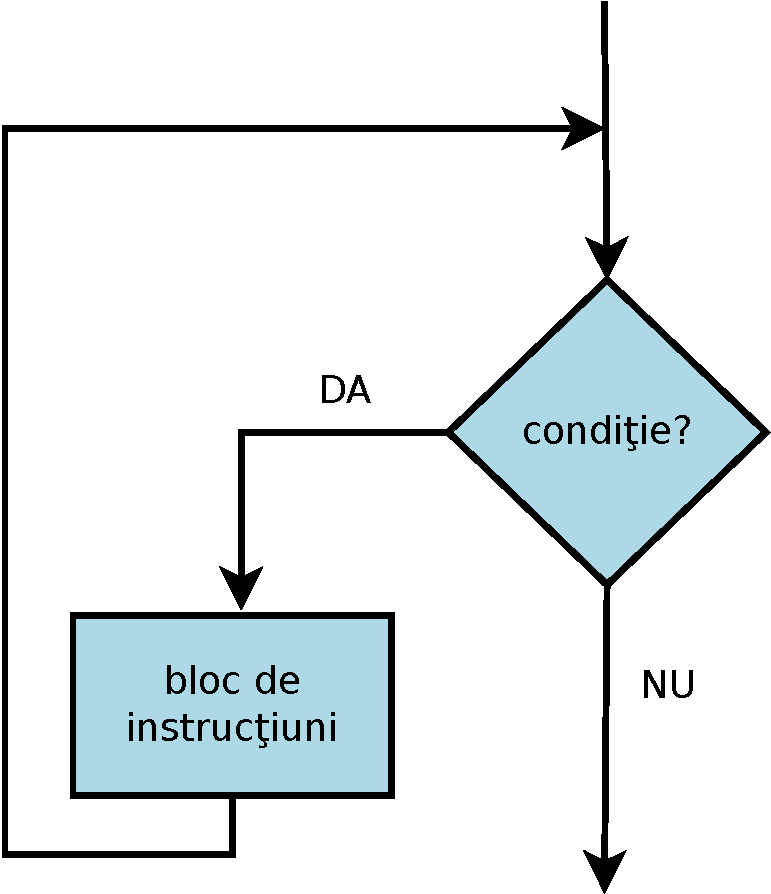
\includegraphics[scale=.5]{cap02/while-crop.pdf}
  \caption{Flowchart buclă while}
  \label{fig:flowchart while loop}
\end{figure}

Dacă condiţia este din start falsă, atunci se continuă execuţia liniară ({\glqq}în jos{\grqq}),
altfel se trece prin blocul de instrucţiuni (care bineînţeles că poate
conţine mai multe instrucţiuni, sau chiar alte bucle, constructe if/else, switch, ş.a.m.d.).
După ce instrucţiunile au fost executate, se ajunge iar la verificarea condiţiei,
şi povestea o poate lua de la capăt.

\attention{Blocul de instrucţiuni trebuie să modifice cumva valoarea de adevăr
a condiţiei care urmează a fi verificate. Altfel riscăm să creăm o buclă
infinită, din care fluxul de execuţie nu va ieşi niciodată.

La acest lucru se ajunge de obicei folosind cel puţin o variabilă în condiţie,
a cărei valoare se schimbă în blocul de instrucţiuni.}

De exemplu, putem număra de la unu la zece, din unu în unu. Pentru asta,
valoarea de start este evident 1. Această valoare o vom salva într-o variabilă.
La fiecare rulare a buclei, adunăm 1 la valoarea variabilei, şi salvăm
rezultatul în aceeaşi variabilă. Astfel avansăm de la 1 la 2, de la 2 la 3,
ş.a.m.d., până la 10. Condiţia de oprire va fi ca valoarea variabilei să
fie mai mică sau egală cu 10. Dacă condiţia nu este adevărată, atunci fluxul de execuţie
{\glqq}trece peste{\grqq} blocul while, şi se continuă execuţia liniară.

Schema logică ar arăta ca în figura \ref{fig:while counting}.

\begin{figure}[h!]
  \centering
    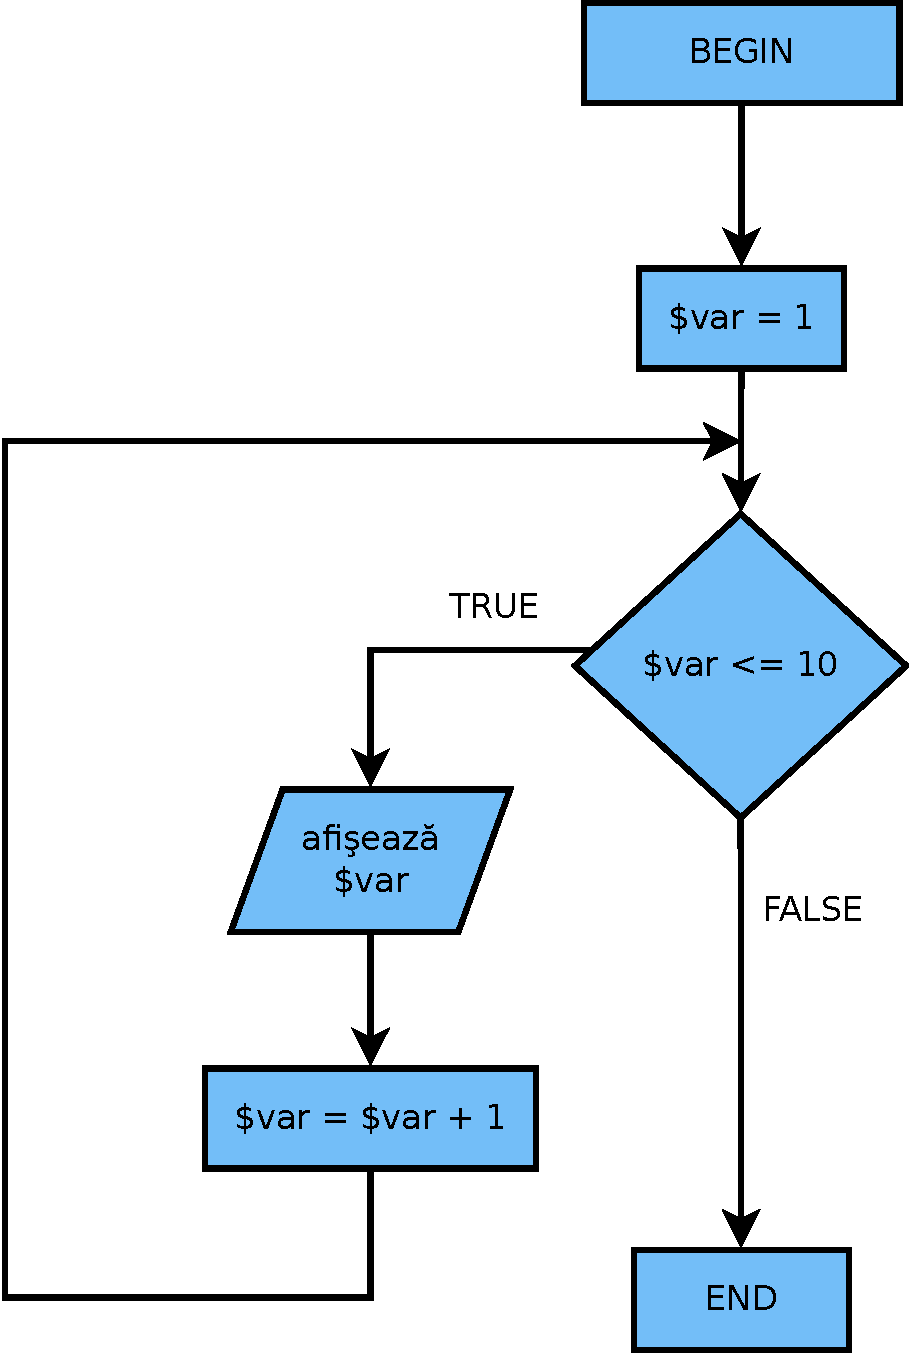
\includegraphics[scale=.5]{cap02/count-while-crop.pdf}
  \caption{Numărând de la 1 la 10}
  \label{fig:while counting}
\end{figure}

\begin{Exercise}[title={Numărătoarea din 1 în 1 cu while},difficulty=1]
\ExePart
Implementează algoritmul din figura \ref{fig:while counting} în limbajul PHP.

\ExePart
Întrebare capcană: Ce valori va lua pe rând variabila \$var?
\end{Exercise}

\texttt{Do while} este foarte asemănătoare cu bucla \texttt{while},
diferenţa fiind că blocul de instrucţiuni va fi executat cel
puţin o dată. Ceea ce este logic, din moment ce mai întâi se
trece prin blocul de instrucţiuni, apoi este verificată condiţia, şi
dacă aceasta este TRUE, atunci se sare înapoi, la începutul blocului de
instrucţiuni.

În altă ordine de idei, iniţial blocul de instrucţiuni
face parte din execuţia liniară. Abia apoi se va decide, în funcţie de valoarea
de adevăr a condiţiei, dacă se va crea o buclă sau nu. Din asta deducem
că fluxul de execuţie poate trece prin {\glqq}bucla{\grqq} \texttt{do while} fără
a face nicio buclă de fapt, fără a sări înapoi nici măcar o dată. Asta s-ar putea
întâmpla dacă condiţia ar fi din start falsă. Însă în contrast cu bucla
\texttt{while}, blocul de instrucţiuni al buclei \texttt{do while} va fi executat cel
puţin o dată.

\begin{Exercise}[title={Schema logică a buclei do while},difficulty=1]
Modifică schema logică generală a buclei \texttt{while} din
figura \ref{fig:flowchart while loop}, transformând-o în
schema logică a buclei \texttt{do while}.
\end{Exercise}


\begin{Exercise}[title={Numărătoarea din doi în doi cu do while},difficulty=1]
\ExePart
Scrie un program care să numere descrescător din 2 în 2, începând de la 23
şi terminând cu un număr negativ la alegere, folosind bucla do while.

\ExePart
Ce face programul tău şi nu este în cerinţă?
\end{Exercise}

\begin{Exercise}[title={Par sau impar?},difficulty=2]
Alege un număr pozitiv nenul N şi scrie un program care
pentru toate numerele din intervalul [-N;N] afişează dacă acestea sunt pare
sau impare. Pentru N=42, outputul va arăta astfel:
\begin{verbatim}
-42 este par
-41 este impar
-40 este par
...
0 este par
...
41 este impar
42 este par
\end{verbatim}
Valorile constante 'este', 'par' şi 'impar' trebuie să apară o singură dată în
cod, iar codul trebuie să facă uz de operatorul ternar şi de operatorul modulo.
\end{Exercise}

\subsection{break şi continue}
Constructul \texttt{break} l-am întâlnit deja în folosirea constructului
\texttt{switch}. Însă \texttt{break}, după cum îi sugerează şi numele, poate
mai mult: poate întrerupe orice buclă.\footnote{A nu se înţelege că \texttt{switch} ar fi o buclă -- nu este}
Fluxul de execuţie din buclă pur şi simplu
va sări din interiorul buclei în afara ei, continuând fluxul liniar
de după buclă.

Unul din scenariile în care avem nevoie de el ar putea fi căutarea:
căutăm un element într-o buclă, şi atunci când l-am găsit, întrerupem
căutarea -- nu ar mai avea rost să terminăm de iterat tot setul de date.

De exemplu, dându-se un număr întreg N ca input, vrem să aflăm următorul
multiplu de 10. Am putea face asta în felul următor:

\begin{lstlisting}
<?php
$n = 231;

while(TRUE === TRUE) {
  if(0 === $n%10) {
	  break;
  }
  $n += 1;
}

echo 'N rotunjit prin adaugire este ',$n;
\end{lstlisting}

Linia 4 ne-ar putea părea ciudată, şi într-adevăr este.
Ea transformă automat bucla while într-una infinită,
deoarece, în mod evident, valoarea de adevăr a comparaţiei nu se va schimba
niciodată. Însă acest lucru este voit, deoarece practic întrerupem
bucla fluxului de execuţie folosind break.

\attention{Dacă nu înţelegi
linia 5, atunci cel mai probabil nu ai sintetizat destul
la ce este util restul operaţiei de împărţire, şi deci
operatorul modulo, prezentat la pagina \pageref{term:modulo}.}

\good{Revizuieşte lecţia \textit{Teorema împărţirii cu rest},
învăţată la matematică în clasa a V-a.}

\begin{Exercise}[title={Majoritatea buclelor infinite pot fi corectate}]
Rescrie codul anterior mutând (şi eventual modificând) condiţia
de întrerupere a buclei (deci condiţia din \texttt{if}),
şi renunţând complet la folosirea \texttt{break}.

Ce crezi, codul este acum mai curat sau nu?
\end{Exercise}

Constructul \texttt{continue} ne permite să
sărim peste restul instrucţiunilor următoare
din ciclul curent al buclei, trecând la ciclul următor.

De exemplu, putem afişa doar numerele care sunt multiple
de trei, şi calcula suma celorlalte numere din intervalul
de numere [0,50] astfel:
\begin{lstlisting}
<?php
$n = 0;
$sum = 0;
while($n <= 50) {
  if(0 === $n%3) {
	  echo $n,' ';
	  $n += 1;
	  continue;
  }
  $sum += $n;
  $n += 1;
}
echo 'Suma este ',$sum;
\end{lstlisting}
Datorită liniei 8, fluxul de execuţie va sări înapoi pe linia 4.
Deoarece la următoarea iteraţie a buclei nu vrem să intrăm cu aceeaşi valoare pentru \$n,
căci ne-am alege cu o buclă infinită, adăugăm 1 la valoarea lui \$n, şi
salvăm rezultatul tot în \$n pe linia 7, înainte de a face saltul înapoi la verificarea
condiţiei.
 

\section{Tipul de date array. Bucla foreach}
Până acum am lucrat doar cu \textsl{tipuri de date scalare}: string, int, float, bool.
Un array este un tip de date \textsl{compozit} şi poate fi folosit în cele mai
diverse situaţii, motiv pentru care este foarte versatil.

Pentru a iniţializa un array, atribuim valoarea \texttt{array()} unei variabile.
Aceasta va conţine un array gol. Exemplu:
\begin{lstlisting}
<?php
$a = array();
var_dump($a);
var_dump(array());
\end{lstlisting}
Din asta deducem că \texttt{array()} poate fi la fel de bine o expresie,
deci poate fi folosit aşa cum am folosit orice altă valoare de până acum,
precum TRUE, 42, sau 'foo':
\begin{lstlisting}
<?php
$a = array();
var_dump($a === array());
if($a === array()) {
  echo '$a este un array gol';
}
\end{lstlisting}

În loc de a compara o variabilă cu \texttt{array()}, PHP
ne pune la dispoziţie un construct special: \texttt{empty()}.
Acesta, împreună cu variabila din interiorul parantezelor
rotunde, este înlocuit de o valoare booleană. Testează
următorul exemplu:
\begin{lstlisting}
<?php
$a = array();
var_dump(empty($a));
\end{lstlisting}
Concluzionăm că \texttt{empty()} poate fi folosit oriunde
am folosit până acum expresii logice, de exemplu în if:

\begin{lstlisting}
<?php
$a = array();
if(TRUE === empty($a)) {
  echo '$a este gol';
}
else {
  echo '$a este plin';
}
\end{lstlisting}

Pentru a iniţializa un array cu elemente în el, le putem
pune între parantezele rotunde ale lui \texttt{array()},
separându-le unul de altul prin virgulă:
\begin{lstlisting}
<?php
$a = array(42,'foo',TRUE,FALSE);
if(TRUE === empty($a)) {
  echo '$a este gol';
}
else {
  echo '$a este plin';
}
\end{lstlisting}
Sper că acum este evident de ce un array este un tip de
date compozit: în el poţi salva alte valori de diferite tipuri
de date.

Exact, un array salvează în el valori precum cele constante
de mai sus. Putem chiar şi copia valorile altor variabile
în array:
\begin{lstlisting}
<?php
$foo = 'bar';
$a = array(42,$foo);
\end{lstlisting}
\attention{Este incorect să spui că variabila \texttt{\$foo} este în array-ul \texttt{\$a}. Nu
variabila este într-un array, ci valoarea acesteia. A doua linie se citeşte deci
astfel: \textit{Copiază valoarea constantă 42 şi valoarea variabilei \texttt{\$foo} într-un array,
şi atribuie array-ul rezultat variabilei \$a}.}

După ce avem un array, vom vrea să prelucrăm valorile
salvate în el într-o buclă, fiecare element pe rând.

Deoarece array-urile sunt foarte importante, PHP
ne pune la dispoziţie încă o buclă, special gândită
pentru ceea ce numim \textsl{iterarea array-urilor}.
Bucla se numeşte \texttt{foreach}.

Sintaxa generală arată astfel:
\begin{verbatim}
foreach(<array>  'as' <value>) {
  <bloc-de-instructiuni>
}
\end{verbatim}
<array> este array-ul pe care vrem să-l iterăm, <value>
este o variabilă inventată de noi care există
doar în interiorul buclei şi care va lua pe rând
valorile păstrate în array, la fiecare iteraţie a buclei.

Să zicem că avem o listă de nume, şi vrem să le afişăm pe toate
unul sub altul, în HTML:
\begin{lstlisting}
<?php
$names = array('Mircea','Claudiu','Ioana','Flavius');

foreach($names as $name) {
  echo 'Salut ', $name,'!<br>';
}
echo 'Hooray!';
\end{lstlisting}

\begin{Exercise}[title={Meniu de navigare},difficulty=1]

\ExePart

Scrie un cod care pornind de la un array precum
\begin{lstlisting}
$menu = array('Home','Contact','Despre');
\end{lstlisting}
generează un meniu de navigare (tag-urile \texttt{<ul>} şi \texttt{<li>}).
Structura codului HTML va trebui să arate astfel:
\begin{verbatim}
<ul>
        <li><a href="#Home">Home</a></li>
        <li><a href="#Contact">Contact</a></li>
        <li><a href="#Despre">Despre</a></li>
</ul>
\end{verbatim}

\ExePart
Îmbunătăţeşte codul astfel încât dacă \texttt{\$menu} este iniţializat gol, astfel:
\begin{lstlisting}
$menu = array();
\end{lstlisting}
să nu mai genereze un meniu, ci output-ul:
\begin{verbatim}
Meniu inexistent.
\end{verbatim}
Pentru asta va trebui să verifici dacă array-ul este gol cu \texttt{empty(\$menu)}, dacă
nu, să faci ceea ce ai făcut în partea I a exerciţiului, altfel să generezi
outputul 'Meniu inexistent'.
\end{Exercise}
Exerciţiul \textit{Meniu de navigare} ţi-a introdus subtil avantajele
array-urilor. Este adevărat că la început codul va fi mult mai
complex decât un meniu static în HTML, însă după ce ai codul, şi
acesta funcţionează, nu trebuie decât să modifici valorile salvate
în array, într-un loc {\glqq}central{\grqq}, şi PHP va genera mereu meniul HTML corespunzător.
Nu vei mai avea de-a face cu HTML direct, nu mai mult decât ai descrie un singur element
\texttt{<li>}, un singur element \texttt{<ul>} sau un singur element \texttt{<a>}.
Asta este posibil mulţumită proprietăţii unei bucle de a repeta un bloc de instrucţiuni.

Ceea ce am făcut în exerciţiul anterior
se numeşte \textit{inventarea unei structuri de date abstracte} (în cazul
nostru este un array, pe care
l-am salvat în \texttt{\$menu}) care emulează ceea ce cunoaştem ca fiind un {\glqq}meniu{\grqq} în {\glqq}viaţa reală{\grqq}.
Deşi nu este el însuşi un meniu, conţine toate datele de care avem nevoie
pentru a genera dinamic un meniu, cu PHP. Aceste date se numesc \textsl{metadate},
concept pe care l-ai cunoscut la începutul acestui capitol.

\attention{După cum ţi-am spus încă de la începutul capitolului, şi după
cum tocmai ai văzut, toate aplicaţiile conţin metadate. Ele vin
deseori {\glqq}împachetate{\grqq} în structuri de date abstracte precum array-ul
salvat în \texttt{\$menu}.}
\good{Obişnuieşte-te cu ideea de a trebui să inventezi date abstracte
care conţin metadate.
%Prin introducerea acestor date abstracte codul tău va fi mai flexibil şi mai mentenabil.
Este adevărat,
la început va trebui să investeşti mai mult timp în
conceperea acestor date abstracte, dar pe termen lung avantajele
în termeni de \textit{mentenabilitate}, \textit{flexibilitate} şi \textit{reutilizare}
a codului se vor face simţite.}

După ce un array a fost iniţializat, putem adăuga elemente adiţionale
la sfârşitul său, folosind operatorul \texttt{[]}. Sintaxa generală este:
\begin{verbatim}
$<array>'[]' = <valoare>
\end{verbatim}
Exemplu:
\begin{lstlisting}[label=lst:push_operator,caption={Adăugarea elementelor la sfârşitul unui array}]
<?php
$names = array('Mircea','Claudiu','Ioana','Flavius');
$names[] = 'Ramona';
\end{lstlisting}
Convinge-te, scrie un cod care iterează array-ul rezultat după adăugarea
elementului 'Ramona'.

Până acum, la fiecare iteraţie a array-ului, valoarea curentă era
pusă în variabila de după \texttt{as}. Însă elementele dintr-un array
au şi un index, o ordine. Pentru a ajunge la acest index, \texttt{foreach}
are o sintaxă extinsă:
\begin{verbatim}
foreach(<array> 'as' <index> '=>' <valoare>) {
  <bloc-de-instructiuni>
}
\end{verbatim}

\begin{Exercise}[title={Sintaxa foreach},difficulty=2]
Scrie un program care iterează toate elementele dintr-un array
şi afişează pentru fiecare 'Elementul <I> are valoarea <V>', unde <I>
este indexul, <V> este valoarea.

\attention{Acest exerciţiu îţi testează capacitatea de a înţelege
o specificaţie sintactică şi de a o aplica în practică,
scriind un cod PHP care o respectă.}
\end{Exercise}

După cum ai observat, elementele dintr-un array sunt numerotate
de la zero la N-1, unde N este numărul total de elemente. Din acest motiv,
spunem că un array este \textsl{0-indexed}. Astfel de array-uri se
mai numesc şi \textsl{vectori} sau \textsl{liste}.

Pot exista situaţii în care vrem un anumit element din array, ştiindu-i
indexul. În astfel de cazuri folosim sintaxa următoare pentru a accesa
acel element:
\begin{verbatim}
$<array>'['<index>']'
\end{verbatim}
<index> poate fi orice expresie care are o valore, aşa cum am văzut până acum,
deci asta include şi operaţii matematice:
\begin{lstlisting}
<?php
$names = array('Mircea','Claudiu','Ioana','Flavius');

$index_fata = 2;

echo 'Eu sunt ',$names[3],'<br>';
echo 'Pe fata o cheama ',$names[$index_fata],', inaintea ei este ',
		  $names[$index_fata-1],' iar dupa ea urmeaza ',$names[$index_fata+1];
\end{lstlisting}

Să zicem că avem următoarea situaţie: avem un array de nume,
şi numele nostru şi vrem să afişăm numele imediat după numele nostru.

Am putea proceda în felul următor:
\begin{lstlisting}[caption={Indexurile sunt consecutive},label=lst:increment]
<?php
$names = array('Mircea','Claudiu','Ioana','Flavius');
$me = 'Claudiu';
$after_me = '<nimeni>';

foreach($names as $index => $name) {
  if($name === $me) {
	$after_me = $names[$index+1];
	break;
  }
}

echo 'Dupa mine este ',$after_me;
\end{lstlisting}
Încearcă acest cod. Apoi încearcă să vezi ce se întâmplă dacă variabila
\$me este iniţializată cu ultima valoare din array. Exact, va
spune că indexul \$index+1 nu există, ceea ce e normal.

Pentru a verifica dacă ceva e setat, PHP ne pune la dispoziţie
încă un construct, similar cu \texttt{empty()}: \texttt{isset()}.
Acesta este înlocuit cu o valoare booleană care reflectă
existenţa parametrului pe care i-l pasăm. În cazul nostru,
am folosi \texttt{isset(\$names[\$index+1])}.

\begin{Exercise}[title={O conjuncţie în practică}]
Adaugă conjunctiv condiţia \texttt{isset(\$names[\$index+1])} la condiţia
deja existentă de pe linia 7 din codul anterior.
\end{Exercise}

Însă putem asocia fiecărui element dintr-un array şi
un index explicit. Pentru asta folosim aceeaşi sintaxă ca
în partea de după 'as' din bucla foreach: \texttt{<index> '=>' <value>}.

Iniţializarea unui astfel de array ar arăta astfel:
\begin{lstlisting}
$fructe = array(
		  231	=> 'mere',
		  1		=> 'pere',
		  1001	=> 'alune'
);
\end{lstlisting}
Un array cu \textsl{date asociative} se mai numeşte şi \textsl{dicţionar}. El asociază
indecşii (sau \textsl{cheile}) din stânga, cu valorile din dreapta.

\good{Nu este obligatoriu să formatezi astfel codul, ai fi putut
scrie totul pe o singură linie. Însă e o practică bună să îl
scrii aşa, pentru a fi cât mai lizibil.}

Dacă indexul lipseşte, atunci se ia indexul cel mai mare
existent în array până în acel moment, şi se incrementează cu o unitate.
De exemplu, în codul:
\begin{lstlisting}
$fructe = array(
		  231	=> 'mere',
		  1		=> 'pere',
		  1001	=> 'alune',
				   'piersici',
				   'caise'
);
\end{lstlisting}
elementul cu valoarea 'piersici' va fi asociat automat cu indexul 1002, iar 'caise'
va fi salvat la indexul 1003, deoarece 1002 există deja.

De fapt, un astfel de dicţionar nu este limitat doar la indecşi numerici.
Poţi folosi şi stringuri pentru asocieri. De exemplu, familia mea
ar putea fi abstractizată într-un array astfel:

\begin{lstlisting}
$my_family = array(
  'me' => 'Flavius',
  'father' => 'Adrian',
  'mother' => 'Simona',
  'brother' => 'Daniel'
);
\end{lstlisting}

%TODO spune că se numeşte dicţionar
Folosind însă un array asociativ în loc de un array indexat\footnote{Se subînţelege
că elementele sunt numerotate consecutiv de la 0 la N-1.}, pierdem automat
din consistenţa ordonării datelor. O problemă de genul celei ilustrate în
codul \ref{lst:increment} nu ar mai fi aşa uşor rezolvabilă, deoarece {\glqq}\$index+1{\grqq}
nu ar mai exista.

Aşadar, când trebuie să concepem o structură de date, trebuie să ne gândim
bine dacă este o asociere, sau o înşiruire. Dacă este o asociere, atunci
vom vrea să folosim chei expresive cărora să le asociem informaţii. Dacă
în schimb constatăm că vrem o înşiruire, atunci nu ar trebui să
ne băgăm nasul peste numerotarea indecşilor, şi să îl lăsăm pe PHP
să facă asta pentru noi, în mod consistent, automat.

Deşi cele două moduri în care pot fi folosite array-urile pot fi amestecate,
în această carte vom folosi termenul de \textsl{index} atunci când ne referim la
array-uri ca la liste de elemente numerotate automat, iar termenul de \textsl{cheie} (en. \textsl{key})
atunci când intenţionăm să folosim informaţiile în mod asociativ.

Indiferent de cum folosim array-ul, indexat sau asociativ, putem citi din el şi
scrie în el date folosind operatorul \texttt{[]}, aşa cum am mai văzut:
\begin{lstlisting}
<?php
$posesor = 'Flavius';
$fructe = array('mere');
$fructe[] = 'pere';
$fructe[23] = 'alune';
$fructe['favorit'] = 'capsuni';
$fructe['favoritul lui '.$posesor] = 'piersici';
$fructe[23*4-1] = 'caise';

echo '<pre>';
var_dump($fructe);
echo '</pre>';

echo 'Cele mai tari sunt ',$fructe['favoritul lui Flavius'],'le';
\end{lstlisting}
Exact, chiar şi în interiorul lui \texttt{[]} putem folosi orice expresie,
expresie a cărei valoare este evaluată mai întâi, pentru care PHP
crează o valoare temporară, şi care e folosită ca cheie apoi.

\section{Bucla for}
În unele din exemplele anterioare am iniţializat mai întâi variabile
precum \$sum cu valoarea 0 înainte de intrarea într-o buclă,
iar la fiecare iteraţie am verificat apoi valoarea 
de adevăr a unei expresii booleene (condiţia buclei) şi eventual
am adăugat unu la un număr.

Bucla for ne permite să facem astfel de lucruri mult mai elegant.
Sintaxa generală este
\begin{verbatim}
for(<initialization> ; <condition> ; <expr>) {
  <block-of-instructions>
}
\end{verbatim}
<initialization> este executată o singură dată, înainte ca
fluxul de execuţie să intre în bucla efectivă,
<condition> şi <expr> sunt executate la fiecare iteraţie
a buclei.

Pentru a număra de la 0 la 100 am putea scrie:
\begin{lstlisting}
<?php
for($i=0;$i<=100;$i += 1) {
  echo $i,' ';
}
\end{lstlisting}

Iniţializarea şi expresia pot conţine iniţializări 
respectiv expresii multiple, separate prin virgulă.

\begin{Exercise}[title={Două câte două},difficulty=2]

\ExePart

Scrie un program folosind bucla for cu iniţializări şi expresii
multiple care calculează suma fiecărui număr par de la 0 la 50
cu numărul impar care îl succedă. Altfel spus, 0+1, 2+3,
4+5, \ldots. Output-ul trebuie să arate aşa:
\begin{verbatim}
0 + 1 = 1<br>
2 + 3 = 5<br>
...
50 + 51 = 101<br>
\end{verbatim}
\ExePart
Rescrie programul folosind o singură variabilă.
\end{Exercise}



\section{Completări}
Ultimele lecţii ţi-au prezentat foarte multe
lucruri noi, însă am sărit intenţionat peste multe
noţiuni tocmai pentru că voiam să ai cât de cât
o imagine de ansamblu mai întâi. Această secţiune îţi
va slefui câteva noţiuni deja cunoscute, aducând
şi completări, şi mai ales sfaturi despre
cum să-ţi scrii codul curat, elegant.


\subsection{Stringuri}
Până acum stringurile au fost scrise mereu
între apostrofuri. Acestea se numesc stringuri simple.

În PHP există însă şi stringuri interpretate,
sau mai bine zis \textsl{stringuri interpolate}. Se numesc
aşa deoarece numele variabilelor din interiorul lor
sunt interpretate şi înlocuite de valorile lor.

Astfel, în loc de:
\begin{lstlisting}
<?php
$nume = 'Flavius';
echo 'Salut ',$nume;
\end{lstlisting}
Poţi scrie:
\begin{lstlisting}
<?php
$nume = 'Flavius';
echo "Salut $nume";
\end{lstlisting}

Pe lângă variabile, în stringurile interpolate
mai sunt interpretate şi
aşa-zisele caractere de control. Aceste caractere
sunt mai mult sau mai puţin {\glqq}invizibile{\grqq}. Aceste
caractere încep cu \textbackslash (en. \textsl{backslash}),
şi sunt urmate de ceva, de obicei de un caracter.

De exemplu, până acum ai generat cod HTML,
cel mai probabil apelând de mai multe ori
\texttt{echo}. Însă dacă te-ai uitat la codul
sursă HTML generat, tot acest cod era într-o linie.
Pentru asta am putea pune o linie nouă folosind un astfel
de caracter numit line feed. Încearcă:
\begin{lstlisting}
<?php
echo "Salut\n";
echo "Flavius";
\end{lstlisting}
După cum ştii, HTML nu interpretează liniile noi într-un mod
special.  Însă dacă te uiţi la sursa generată, sau faci
o cerere cu telnet, vei vedea că cele două stringuri 
se află pe linii diferite, unul sub altul. De fapt, nici
nu e nevoie să foloseşti două stringuri constante, poţi
scrie totul într-un cârnat lung:
\begin{lstlisting}
<?php
echo "Salut\nFlavius";
\end{lstlisting}
Deşi nu este un spaţiu între cuvinte, browserul interpretează
corect linia nouă şi afişează un spaţiu între ele, deoarece
aşa dictează formatul HTML.

Un alt caracter special este \texttt{{\textbackslash}t}.
Acesta are acelaşi efect cu apăsarea tastei \keystroke{TAB}.

Deoarece caracterul {\textbackslash} este folosit pentru ceea
ce numim \textsl{escaping}, pentru a afişa caracterul backslash
însuşi trebuie să îl escape-uim şi pe el, deci ne alegem cu
două caractere backslash pentru a reprezenta un singur caracter.
Exemplu:
\begin{lstlisting}
<?php
echo '\ se numeste backslash';
echo "\\ se numeste backslash";
\end{lstlisting}

Caracterul {\textbackslash} este folosit din motive istorice,
ar fi putut fi orice alt caracter.

În exerciţiul \textit{Sintaxa HTML} de la începutul
capitolului, ai pus de exemplu caractere precum '<' între
apostrofuri, tocmai pentru a diferenţa caracterul < care are
o semnificaţie specială în metalimbajul inventat de noi de
caracterul '<' care voiai să fie interpretat exact aşa cum e.
Altfel spus, punând caractere între apostrofuri, am spus
că \textit{acest caracter trebuie {\glqq}scăpat printre degete{\grqq}}, deci
nu trebuie interpretat de metalimbaj, si face parte din input/output.

Pentru a înţelege ce înseamnă acest \textit{scăpat printre degete},
trebuie să înţelegem cum funcţionează parsarea în PHP.\footnote{De fapt,
lexicalizarea, un pas din {\glqq}parsare{\grqq}. Detaliile mai mult l-ar
induce în eroare pe cititor.}

Atunci când PHP {\glqq}execută{\grqq} un script, primul lucru pe care îl
face este să citească fişierul PHP scris de noi, caracter
cu caracter. PHP citeşte rând pe rând caracterele 'e','c','h','o',
şi deoarece recunoaşte acest şir de patru caractere ca fiind
constructul \texttt{echo}, ştie că ce urmează trebuie să
fie o expresie cu o valoare. Altfel spus, {\glqq}echo{\grqq} pune
parserul în \textsl{contextul semantic} de a se aştepta la o
expresie.

Apoi PHP ajunge la caracterul ', şi ştie că urmează
un şir de caractere care trebuie luat ca atare, ca o valoare
constantă. PHP ştie şi că trebuie să citească caractere şi
să le pună în acest string până întâlneşte iar caracterul '.

Hai să vedem ce se întâmplă în cazul următor:
\begin{lstlisting}
echo 'You're online';
\end{lstlisting}
PHP citeşte {\glqq}echo{\grqq}, vede spaţiul şi îl acceptă pe {\glqq}echo{\grqq}
ca construct al limbajului, apoi vede ' şi începe să
pună, caracter cu caracter, literele Y,o,u într-un nou string.
Apoi, deoarece a întâlnit încă o dată ', şi deoarece tocmai se află
deja in contextul semantic al unui string, PHP îşi dă seama că
acesta e sfârşitul stringului. Altfel spus, PHP ar executa asta:
\begin{lstlisting}
echo 'You'
\end{lstlisting}
Problema este că la sfârşitul instrucţiunii PHP se aşteaptă să
vadă ori ',', ori ';', deci se blochează la
\begin{lstlisting}
re online';
\end{lstlisting}
care nu e o instrucţiune validă nici măcar din punct
de vedere sintactic.

În interiorul stringurilor
simple, delimitate de apostrofuri, caracterul ' are semnificaţia
specială de a termina însuşi stringul.
Escaping înseamnă să-l forţăm pe PHP să {\glqq}scape printre degete{\grqq}
aceste caractere speciale. Pentru a face escaping, vom precede caracterul
special cu \textbackslash:
\begin{lstlisting}
<?php
echo 'You\'re online';
\end{lstlisting}
Astfel PHP, atunci când întâlneşte \textbackslash, ştie că
următorul caracter nu trebuie interpretat într-un {\glqq}mod special{\grqq},
ci doar adăugat la stringul pe care tocmai îl citeşte.

În astfel de cazuri poţi însă să foloseşti stringuri interpretate,
deoarece în interiorul lor caracterul ' nu mai are semnificaţia de
delimitator:
\begin{lstlisting}
<?php
echo "You're online";
\end{lstlisting}

Similar, atunci când vrei să construieşti un string care conţine
cod HTML, mult mai curat este:
\begin{lstlisting}
echo '<form method="post">';
\end{lstlisting}
decât:
\begin{lstlisting}
echo "<form method=\"post\">";
\end{lstlisting}



Vor exista cazuri în care vei fi nevoit să salvezi stringuri constante
foarte largi într-o variabilă, sau să afişezi o astfel de valoare.

Pentru astfel de cazuri există două tipuri de stringuri: \textsl{nowdoc} şi \textsl{heredoc}.
Cele dintâi se manifestă exact ca stringurile simple, cele din urmă
sunt stringuri interpolate.

Stringurile nowdoc sunt introduse de operatorul  \verb '<<<' urmat de un string neinterpretat.
Acest string va fi folosit de PHP ca marcaj pentru a determina sfârşitul stringului. Marcajul de sfârşit trebuie
să apară pe o singură linie şi să fie primul şi singurul lucru pe acea linie, fără a fi precedat nici măcar
de spaţii, şi urmat doar de ';'. Exemplu concret:

\begin{lstlisting}
echo <<<'EOD'
  $foo este o variabila 
EOD;
\end{lstlisting}

Bineînţeles că poţi atribui valoarea unei variabile, sau face orice
alte operaţii cu un astfel de string:
\begin{lstlisting}
<?php
$bar = <<<'EOD'
  $foo este o variabila
EOD;
\end{lstlisting}

Sintaxa heredoc pentru stringurile interpolate este foarte asemănătoare:
\begin{lstlisting}
<?php
$foo = 'bar';
echo <<<EOD
  $foo este o variabila 
EOD;
\end{lstlisting}

Avantajele heredoc şi nowdowc faţă de stringurile interpolate sau simple este că
caracterele " respectiv ' pot fi folosite fără niciun fel de restricţie.

\subsection{Constante şi alte tipuri de date}
În PHP există câteva constante predefinite pe care PHP le
crează automat pentru noi. Constantele urmează aceleaşi
standarde de denumire ca şi variabilele, cu două excepţii:
\begin{itemize}
	\item identificatorul constantei nu este precedat de simbolul \$
	\item constantele definite de programator nu trebuie să înceapă cu două caractere
underscore, deoarece acestea sunt rezervate pentru adăugiri viitoare în limbaj
\end{itemize}
Sintaxa definirii unei constante este
\begin{verbatim}
const <identificator> = <valoare>;
\end{verbatim}
\texttt{<valoare>} poate fi orice expresie care evaluată, rezultă într-o valoare,
de orice tip ar fi aceasta: int, float, string, sau bool. Array-urile, fiind un tip
de date compozit, nu poat fi salvate în constante.

O constantă, aşa cum îi spune şi numele, nu îşi poate schimba valoarea o dată
ce a fost definită. Constantele sunt evaluate ca expresii, deoarece au valori,
ca şi variabilele. Exemple:
\begin{lstlisting}
<?php
const NUME = 'Flavius';

echo 'Salut ',NUME;
echo ' Ce faci '.NUME.'?';
\end{lstlisting}

PHP îţi pune la dispoziţie multe constante predefinite, însă doar
câteva sunt de interes general
pentru noi deocamdată.

Fiecare sistem de operare  are o reprezentare proprie
a caracterului {\glqq}linie nouă{\grqq}. Windows foloseşte {\glqq}{\textbackslash}r{\textbackslash}n{\grqq} (o
serie de două caractere{\glqq}), Linux are {\grqq}{\textbackslash}n" iar Macintosh foloseşte
{\glqq}{\textbackslash}r{\grqq}. Constanta PHP\_EOL va avea mereu valoarea corectă pentru
fiecare sistem de operare.

Alte constante predefinite de interes general sunt PHP\_VERSION, PHP\_OS,
PHP\_SAPI, PHP\_INT\_MAX -- valoarea maximă a unui număr întreg, INF pentru
reprezentarea infinitului, NAN (en. \textsl{not a number}) pentru valori
care nu sunt numere.

Există câteva constante magice în PHP. Acestea îşi schimbă valoarea
în funcţie de context. Pentru noi interesante sunt deocamdată
\_\_LINE\_\_ pentru linia curentă, \_\_FILE\_\_ pentru fişierul
curent, şi \_\_DIR\_\_ pentru directorul în care se află fişierul curent.
\_\_LINE\_\_ este foarte util pentru a determina prin ce linii 
a trecut fluxul de execuţie, şi deci pentru a depana (en. \textsl{debugging})
logica scriptului. Exemplu:
\begin{lstlisting}
<?php
echo 'PHP incepe executia scriptului "',__FILE__,'"<br />';
$test = TRUE;
echo 'Fluxul de executie trece prin linia ',__LINE__,'<br />';
if(TRUE === $test) {
  echo 'Fluxul de executie trece prin linia ',__LINE__,'<br />';
}
else {
  echo 'Fluxul de executie trece prin linia ',__LINE__,'<br />';
}
echo 'Fluxul de executie trece prin linia ',__LINE__,'<br />';
\end{lstlisting}

Există încă un tip fundamental de date în PHP: NULL. Tipul NULL
este pentru iniţializarea variabilelor care pot lua valori diferite, de tipuri
diferite, şi pentru care nu ştim a priori ce tip de date vor avea.

NULL mai este bun şi pentru iniţializarea variabilelor care urmează să fie
stringuri, şi vrem să ne asigurăm că acea variabilă va exista.

NULL este util şi pentru a semnaliza că o variabilă are o valoare invalidă.
De exemplu, lucrăm la un magazin online şi îi cerem utilizatorului să
introducă numărul de bucăţi dorite. Iniţializăm variabila cu NULL,
pentru a ne asigura că aceasta va exista, indiferent de ce va introduce
utilizatorul, apoi
citim inputul. Dacă utilizatorul nu introduce o cantitate, noi vedem că
variabila încă are valoarea NULL, lucru din care deducem că utilizatorul
nu a introdus o cantitate, deci afişăm o eroare. La un minim, un astfel
de algoritm ar arăta astfel:
\begin{lstlisting}
$cantitate = NULL;
//nu stim inca cum sa citim input, dar hai sa presupunem
//ca urmatoarea linie pune in mod magic valoarea introdusa in variabila
//$cantitate = $input;
if(NULL !== $cantitate) {
  echo "Ati comandat $cantitate bucati";
}
else {
  echo 'Eroare: trebuie sa introduceti o cantitate';
}
\end{lstlisting}

De fapt, NULL, TRUE şi FALSE sunt constante în PHP, numai că sunt
{\glqq}întâmplător{\grqq} susţinute în mod {\glqq}oficial{\grqq} de PHP.

\subsubsection{Type casting şi convertirea implicită}
Type casting înseamnă a converti o variabilă care are o valoare
de un tip de date într-o valoare de un alt tip de date. Pentru asta
punem noul tip de date în paranteze, urmat de valoarea pe care vrem
să o convertim. Spunem că am convertit explicit valoarea dintr-un tip
de date în altul. Exemplu:
\begin{lstlisting}[label=lst:typecasting,caption=Type casting explicit]
<?php
var_dump(5);
var_dump( (string)5 );
var_dump('TRUE');
var_dump( (bool)'TRUE' );
var_dump( (bool)'' );
var_dump( (string)array() );
var_dump( (bool)array() );
var_dump( (bool)array('') );
$test = (float)'FALSE';
var_dump($test);
var_dump( (bool)5);
var_dump( (bool)0);
var_dump( (bool)-42);
\end{lstlisting}

\begin{Exercise}[title={Observaţii type casting},difficulty=1]
Explică în limba română, cu cuvinte proprii, tot ce observi în codul de mai sus.

Ce valori şi de ce tipuri de date rezultă în ce valori convertite în ce
tipuri de date?

Ce valori sunt evaluate ca TRUE, şi ce valori ca FALSE?
\end{Exercise}

Unele valori sunt evaluate ca FALSE atunci când sunt sunt folosite în
contextul unei expresii booleene. Spunem că o valoare este convertită
implicit. Dacă până acum am scris:
\begin{lstlisting}
<?php
$test = TRUE;
if(TRUE === $test) {
  echo 'este adevarat';
}
\end{lstlisting}
mult mai scurt ar fi fost:
\begin{lstlisting}
<?php
$test = TRUE;
if($test) {
  echo 'este adevarat';
}
\end{lstlisting}
Deoarece valoarea variabilei \$test este convertită automat în tipul bool, aşa cum ai văzut
în listingul \ref{lst:typecasting}.

Automat sunt convertite şi valorile numerice (int şi float) care sunt de fapt stringuri, atunci
când aceste stringuri sunt folosite în contextul unor operaţii matematice:
\begin{lstlisting}
<?php
$foo = '3.14';
$bar = '2';
echo $foo * ($bar + 3);
\end{lstlisting}
\bad{Este greşit să salvezi valori numerice ca stringuri, să faci operaţii
matematice cu aceste stringuri şi să te bazezi pe PHP că va face conversiile automat.
Valorile pe care le salvezi în variabile sau în constante trebuie să reflecte
tipul lor de date.}


\subsection{Alţi operatori}
Deseori am fost nevoiţi să adăugăm sau să scădem 1 la o variabilă. Aceste operaţii
se numesc a \textsl{incrementa} respectiv a \textsl{decrementa} o variabilă.

Iniţial am făcut asta explicit, aşa:
\begin{lstlisting}
$foo = $foo + 1;
\end{lstlisting}
Apoi am văzut că putem uni o operaţie matematică cu operaţia de atribuire, şi am folosit:
\begin{lstlisting}
$foo -= 1;
\end{lstlisting}
Aceste operaţii sunt foarte des întâlnite, în special în bucle (predominant în for, dar şi
în alte bucle), deci avem doi operatori speciali pentru asta: ++ pentru incrementare şi
\verb --  pentru decrementare.
\begin{lstlisting}
<?php
$foo = 42;
$foo++;
$foo--;
echo $foo,PHP_EOL;
\end{lstlisting}

Aceşti doi operatori pot fi puşi atât în faţa variabilei, cât şi în urma sa, aşa
cum am făcut în exemplul de mai sus. Când sunt puşi în faţa variabilei, se numesc
operatori de \textsl{preincrement} respectiv \textsl{predecrement}. Când sunt puşi
după variabilă, ei poartă numele de \textsl{postincrement} respectiv \textsl{postdecrement}.

Diferenţa dintre post- şi pre- poate fi evidenţiată cu echo:
\begin{lstlisting}
<?php
$the_answer = 42;
echo $the_answer++,' ';
echo $the_answer;
\end{lstlisting}
Linia 3 mai întâi evaluează variabila, o afişează cu echo, şi apoi
o incrementează. Faptul că într-adevăr variabila a fost incrementată
se vede pe linia 4.

În schimb, în cazul operaţiei {\glqq}pre-{\grqq}, mai întâi se face incrementarea sau decrementarea,
şi apoi rezultatul este pasat lui echo:
\begin{lstlisting}
<?php
$the_answer = 42;
echo ++$the_answer,' ';
echo $the_answer;
\end{lstlisting}

\begin{Exercise}[title={Decrementarea într-o buclă},difficulty=1]
\ExePart
Explică ce face următorul algoritm pas cu pas şi ce reprezintă rezultatul final.
\begin{lstlisting}
<?php
$the_answer = 42;
$foo = 0;
while($the_answer--) {
  $foo += $the_answer;
}
echo $foo;
\end{lstlisting}
\ExePart
Modifică codul din partea I astfel încât să folosească operatorul predecrement în loc de postdecrement,
însă rezultatul afişat să fie acelaşi.
\end{Exercise}

\subsection{Sfaturi de stil}
Ceea ce ai pus la bucle precum while, do while, for, foreach sau constructe
precum if/else/elseif/switch între acolate (\{ şi \}) se numeşte un bloc de instrucţiuni.

Dacă un bloc de instrucţiuni consistă dintr-o singură instrucţiune, atunci folosirea
acoladelor pentru a delimita blocul de instrucţiuni nu este necesară. Astfel, secvenţe
de cod precum
\begin{lstlisting}
if($is_admin) {
  echo 'administrator';
}
\end{lstlisting}
şi
\begin{lstlisting}
<?php
if($is_admin)
  echo 'administrator';
\end{lstlisting}
sunt complet echivalente din punct de vedere funcţional.

\bad{Crearea de blocuri de instrucţiuni fără acolade, ca în exemplul
anterior, este o practică proastă. Deseori se întâmplă să adaugi
o nouă instrucţiune, dar să uiţi să adaugi acoladele, ceea
ce poate duce la bug-uri greu de identificat.

Deci e mai bine să scrii codul din prima cu acolade chiar şi
acolo unde nu sunt necesare, pentru a te feri de frustrările
cauzate de propriile tale greşeli. Şi cu toţii putem
face astfel de greşeli, mai ales când suntem sub presiunea
timpului sau suntem obosiţi.

Totuşi două apăsări de taste nu costă mult, iar avantajele primite
merită efortul.}

O altă tactică de a te feri de propriile greşeli este să compari o constată
cu o variabilă, nu o variabilă cu o constantă. Astfel, oricât de obosit
sau neatent ai fi, nu vei putea face greşeli de genul
\begin{lstlisting}
<?php
$rol = 'user';
if($rol = 'admin') {
  echo 'esti admin';
}
\end{lstlisting}
Linia 3 ar fi executată astfel: \textit{atribuie valoarea 'admin' variabilei
\$rol, şi apoi verifică dacă variabila \$rol este evaluată ca TRUE}.

După cum ai văzut în listingul \ref{lst:typecasting}, orice string diferit
de '' este evaluat boolean ca TRUE, deci fluxul de execuţie va trece mereu
prin blocul de instrucţiuni al if-ului. Mult mai bine ar fi să scriem:
\begin{lstlisting}
<?php
$rol = 'user';
if('admin' = $rol) {
  echo 'esti admin';
}
\end{lstlisting}
În astfel de cazuri, PHP ne va avertiza că nu putem atribui valoarea variabilei
\$rol unei valori constante precum 'admin'. Aceeaşi tehnică funcţionează nu numai
pentru valori constante, ci şi pentru \textsl{constante simbolice} declarate cu cuvântul
cheie \texttt{const}.

Un alt sfat este să nu introduci variabile sau constante noi decât atunci când
acestea chiar îşi au rostul. Scopul unei variabile este să salveze în ea
valori variabile, ce se pot schimba în timpul execuţiei. Dar asta nu e tot.
Nu ar trebui să copiezi valorile unor variabile în alte variabile doar
de dragul de a o face. De exemplu, astfel de atribuiri nu îşi au rostul:
\begin{lstlisting}
$nume = $input;
\end{lstlisting}
deoarece \$input conţine deja inputul. Atribuirea ar avea rost doar dacă ai face
şi o validare, de exemplu cu type casting:
\begin{lstlisting}
$cantitate = (int) $input;
\end{lstlisting}
În astfel de cazuri nu copiezi pur şi simplu valoarea dintr-o parte în alta, ci
o şi validezi, deci nu este o {\glqq}copie perfectă{\grqq}.

În afară de asta, copierea fără sens a unor valori dintr-o variabilă în alta mănâncă
memorie RAM degeaba, care de obicei e limitată.

\subsection{Breaking down the logic}
Fie conjuncţia \texttt{A \&\& B}. Avem următorul tabel de adevăr:

\begin{table}[h!]
  \begin{center}
  \begin{tabular}{cccc}
  Cazul nr & \textbf{A} & \textbf{B} & \textbf{A $\land$ B}\\
  1 & T & T & T\\
  2 & T & F & F\\
  3 & F & T & F\\
  4 & F & F & F
  \end{tabular}
  \end{center}
  \caption{Tabelul adevărului pentru conjuncţii}
  \label{tbl:truth table and}
\end{table}

Însă această conjuncţie folosită cu constructele \texttt{if} şi
\texttt{else} nu poate face diferenţa între ultimele 3 cazuri dintre
cele 4 din tabelul anterior: toate vor fi acoperite de ramura \texttt{else}:

\begin{lstlisting}[mathescape]
if(A && B) {
  //cazul T $\land$ T = T
}
else {
  //cazurile 2, 3, 4
}
\end{lstlisting}
Ce facem însă dacă vrem să tratăm fiecare dintre cele 4 cazuri individual?
Simplu: ne folosim de faptul că \textit{dacă A şi B} este acelaşi lucru ca
\textit{dacă A şi dacă B}, rescriind exemplul nostru astfel:
\begin{lstlisting}[mathescape]
if(A) {
  if(B) {
    //cazul T $\land$ T = T (cazul 1)
  }
  else {
    //cazul T $\land$ F = F (cazul 2)
  }
}
else {
  //once we're on this branch, we know that A is FALSE, but what about B?
  if(B) {
    //cazul F $\land$ T = F (cazul 3)
  }
  else {
    //cazul F $\land$ F = F (cazul 4)
  }
}
\end{lstlisting}

\begin{Exercise}[title={Breaking down the logic of a disjunction},difficulty=1]
Crează tabelul de adevăr al disjuncţiei $A \lor B$ şi rupe-i logica în părţile
componente după tabelul creat, ca în exemplul anterior.
\end{Exercise}

\subsection{Coding convention}
\textsl{Coding convention} este un set de reguli de formatare a codului sursă
şi de numire a identificatorilor variabilelor, funcţiilor sau constantelor.

Având un astfel de set de reguli pe care toţi programatorii îl respectă, codul
sursă devine mai uşor de înţeles şi mentenat.

Există câteva standarde larg răspândite, majoritatea având diferite viziuni
despre ce înseamnă {\glqq}cod uşor de înţeles şi mentenat{\grqq}.

Şi \textit{Yet Another Project}\footnote{\url{http://yet-another-project.com/}}
are un astfel de standard. Acesta
%FIXME finish this


\section{Input şi formulare}
Atunci când utilizatorul introduce date, pe care le numim colectiv \textsl{input},
acele date trebuie salvate în ceva pentru a avea acces la acele date. Iar cel
mai la îndemână loc de a le salva sunt variabilele.

Una dintre variabilele în care PHP salvează automat un anumit tip de input este \get.
Pentru a o popula cu valori, un utilizator trebuie să introducă ceva în \textsl{request line}-ul
cererii HTTP.

Deci crează un script \texttt{get.php} cu următorul conţinut, ca să vezi ce conţine variabila \get:
\begin{lstlisting}
<?php
var_dump($_GET);
\end{lstlisting}
Apoi crează o cerere HTTP cu telnet:
\begin{verbatim}
GET /get.php HTTP/1.1
Host: localhost

\end{verbatim}
Întreaga comunicaţie va arăta cam aşa:
\begin{verbatim}
GET /webdev/get.php HTTP/1.1
Host: localhost

HTTP/1.1 200 OK
Date: Sun, 06 Jun 2010 20:27:40 GMT
X-Powered-By: PHP/5.3.2
Content-Length: 13
Content-Type: text/html

array(0) {
}
\end{verbatim}
Observăm că {\get} este un array, şi că are zero elemente. Altfel spus,
e un array gol. Ceea ce e logic, din moment ce nu pare să fi făcut niciun
pas special pentru a introduce date. Pentru a introduce date cu metoda GET,
trebuie să creăm parametri pe care să-i adăugăm la adresa resursei cerute.
Sintaxa generală este:
\begin{verbatim}
'/path/to/script.php' ['?' <name> '=' <value> ['&' <name> '=' <value>]+ ]
\end{verbatim}
În cuvinte: numele resursei este urmat de semnul întrebării, apoi o serie de
una sau mai multe perechi nume {\glqq}ia valoarea{\grqq} valoare, separate de caracterul
ampersand ('\&').

Deci fă cererea HTTP:
\begin{verbatim}
GET /get.php?foo=bar&answer=42
\end{verbatim}

Vei vedea că \get\ are valoarea:
\begin{verbatim}
array(2) {
  ["foo"]=>
  string(3) "bar"
  ["answer"]=>
  string(2) "42"
}
\end{verbatim}
După cum observi, nu e nimic special la \get, este un array asociativ
cu care putem lucra aşa cum am lucrat cu toate array-urile de până acum.
Cheile din array sunt numele parametrilor, iar valorile \ldots Valorile sunt
mereu stringuri!

Asta nu este neapărat un lucru rău, PHP ne scapă de necesitatea de a converti
(cu type casting) explicit atunci când detectează că poate face o conversie
automată, însă mult mai bine este să convertim noi toate inputurile.

PHP decide cum trebuie să convertească anumite tipuri de date în alte tipuri
de date în funcţie de \textit{contextul semantic} în care punem acele date. De exemplu
o valoare 'ABC' în contextul semantic al unei expresii booleene este evaluată
ca TRUE.

\attention{Pentru a valida cu adevărat inputul, va trebui să folosim funcţii,
însă funcţiile vor fi prezentate abia în capitolul 3. Deci deocamdată ne
prefacem că un simplu type casting şi câteva verificări sunt suficiente.
Facem asta pentru a ne educa din start cu ideea necesităţii validării inputului.

Tehnici de validare complete vor fi prezentate după introducerea funcţiilor.}

Deci vom putea face un calculator care adună două numere a şi b
introduse de utilizator, şi afişează rezultatul adunării:
\begin{lstlisting}
<?php
echo (int)$_GET['a'],' + ', (int)$_GET['b'], ' = ', $_GET['a'] + $_GET['b'];
\end{lstlisting}
Vizitează adresa \texttt{http://localhost/add.php?a=3\&b=4}.

Dar oare ce se întâmplă atunci când unul dintre parametri este inexistent?
Hai să vedem. Vizitează direct \texttt{http://localhost/add.php}. PHP îţi
va spune ce ai greşit. Mesajul în browser este dificil de citit, deci
foloseşte opţiunea {\glqq}view source{\grqq} a browserului tău. În firefox, poţi apăsa
\keystroke{CTRL+U}.

PHP ne spune ceva de genul
\begin{verbatim}
Undefined index: a in add.php on line 2
\end{verbatim}
pentru fiecare acces la indexul (cheia) 'a' respectiv 'b'
de pe linia 2. Astfel de mesaje ar putea fi utile unui
atacator care ar putea deduce din mesajele afişate cam cum
arată codul tău sursă. Ar putea folosi acele deducţii pentru
a-ţi sparge site-ul.

Din acest motiv vrem să verificăm mai întâi
dacă cheile 'a' respectiv 'b' există într-adevăr în \get\ \textit{înainte}
de a accesa acei membri ai array-ului. Dacă ambii membri 'a'
şi 'b' nu sunt prezenţi, atunci afişăm un mesaj de eroare,
altfel facem calculele, pentru că avem cu ce. În acest fel,
orice ar introduce un eventual atacator, acesta nu ar
vedea informaţii importante pentru el pe care noi nu vrem
să le dezvăluim despre codul nostru sursă:
\begin{lstlisting}[label=lst:addition,caption={Un calculator simplu}]
<?php
if(!isset($_GET['a']) || !isset($_GET['b'])) {
  echo 'Introdu a si b.';
}
else {
  echo (int)$_GET['a'],' + ', (int)$_GET['b'], ' = ', $_GET['a'] + $_GET['b'];
}
\end{lstlisting}
După cum ştii, operatorul de negaţie în PHP este !. El inversează practic valoarea
de adevăr a expresiei logice care urmează. În cazul nostru inversează
valoarea de adevăr a constructului isset(),
care are în interior pe rând parametrii \verb|$_GET['a']| respectiv  \verb|$_GET['b']|.
\begin{Exercise}[title={Înţelege expresia logică},difficulty=1]
\ExePart
Cum se citeşte linia 2 din listingul \ref{lst:addition}? Începe răspunsul aşa:\\
\textit{Dacă \ldots}.

\ExePart

Rescrie condiţia într-o formă {\glqq}mai compactă{\grqq} folosind legile lui De Morgan.
Explică încă o dată cum se citeşte această nouă linie de cod, aşa cum
ai făcut în partea I a exerciţiului pentru condiţia iniţială.
\end{Exercise}

\good{Mereu caută să-ţi rescrii expresiile logice cu ajutorul
legilor lui De Morgan astfel încât să conţină cât mai multe conjuncţii logice.
Asta îţi va face scriptul mai rapid, deoarece într-o conjuncţie logică, de îndată
ce s-a întâlnit o valoare FALSE, expresiile următoare din acea conjuncţie
nu mai sunt evaluate, pentru că nu mai are rost: întreaga conjuncţie logică
va avea oricum valoarea de adevăr FALSE.

Deci dacă în exemplul nostru ar fi mai probabil să nu existe 'b', dar să existe 'a',
atunci ar fi mai bine să verificăm mai întâi dacă 'b' este setat. Asta ne-ar economisi
nevoia de a-l verifica şi pe 'a'.

În exemplul nostru micuţ nu este neapărat cazul, şansele statistice ca un
utilizator răuvoitor să nu seteze ori 'a' ori 'b' sunt practic egale. Însă reţine
această modalitate de optimizare pentru situaţiile mai complexe.

De exemplu, de preferat ar fi să verifici mai întâi unele variabile introduse de
utilizator, şi abia apoi să verifici conjunctiv valori dintr-o bază de date, deoarece
operaţiile precum căutările în baze de date sunt mult mai scumpe în termeni
de performaţă.
}

\begin{Exercise}[title={Un calculator complet},difficulty=2]
Crează un script care acceptă doi parametri obligatorii 'a' şi 'b' şi un parametru
opţional 'op' care ia ca valori 'add', 'sub', 'mul', 'div' sau 'mod' pentru fiecare
dintre operaţiile adunare, scădere, înmulţire, împărţire şi modulo.

Dacă parametrul 'op' nu este specificat, atunci trebuie să calculeze rezultatul
tuturor operaţiilor $a+b,a-b,a*b,a/b$ şi $a\%b$ şi să le afişeze rezultatul. Dacă este
specificat, scriptul trebuie să calculeze doar operaţia corespunzătoare şi
să-i afişeze rezultatul.

Foloseşte constructul \texttt{switch} pentru a decide ce operaţie trebuie să faci.
Provocarea constă în a nu scrie cod repetitiv.

\textit{Cod repetitiv} înseamnă că ai o secvenţă de una sau mai multe instrucţiuni identice
în mai multe locuri din algoritm.
\end{Exercise}

\subsection{Formulare, business logic şi view logic}

Însă utilizatorul de rând nu ar trebui să aibă cunoştinţe tehnice pentru a-ţi
trimite date către procesare. Pentru asta există formulare HTML.

Numele câmpurilor de input (atributul \texttt{name}) vor fi folosite \textit{de browser}
pentru a genera URL-ul corect, dacă formularul este
trimis prin metoda GET. De exemplu, un script de întâmpinare a
vizitatorului ar putea arăta astfel:
\begin{lstlisting}
<?php
$mesaj = NULL;
if(isset($_GET['submit'])) {
  if(isset($_GET['nume']) && $_GET['nume']) {
	$mesaj = 'Salut '.$_GET['nume'];
  }
  else {
	$mesaj = 'Eroare: Nu ai introdus numele.';
  }
}
echo $mesaj;
?>
<form method="get">
<label for="nume">Nume:</label>
<input type="text" name="nume" id="nume" />
<input type="submit" name="submit" value="saluta-ma" />
</form>
\end{lstlisting}
Scriptul este constituit din două părţi: liniile 2-10 se ocupă de procesarea
formularului. Liniile 11-17 se ocupă de generarea outputului pe baza datelor
procesate.

Transmiterea de informaţii din procesare către generarea de output se face
folosind \textsl{variabila intermediară} \$mesaj. Deoarece ea va avea ca valoare un
string, o iniţializăm cu valoarea NULL, pe linia 2.

Dacă condiţia de pe linia 3 este adevărată, înseamnă că utilizatorul a apăsat
butonul {\glqq}submit{\grqq}. În acest caz, vrem să procesăm formularul.

Indiferent
dacă formularul a fost trimis sau nu, 
afişăm direct mesajul, care e NULL dacă formularul nu a fost trimis, deci nu rezultă niciun output în
urma executării liniei 11, şi afisăm şi formularul.

Dacă formularul nu a fost trimis, atunci cel mai probabil vizitatorul tocmai a intrat
pe pagina noastră şi urmează să-l completeze şi să-l trimită.

Linia 4 verifică dacă \texttt{\$\_GET['nume']} este setat, şi dacă da, verifică
şi dacă valoarea salvată în el este evaluată boolean ca fiind TRUE. Altfel spus,
verifică şi dacă stringul nu este gol (\texttt{''}) sau nu are valoarea '0'.

Dacă toate acestea sunt adevărate, se generează o valoare dinamică ca mesaj de salut pe linia 5.
Altfel valoarea dinamică va fi un mesaj de eroare, iniţializat pe linia 8.

Procesarea formularului de pe liniile 2-10 se numeşte şi \textsl{business logic}.
Acea secvenţă
din cod validează inputul şi setează variabila intermediară \$mesaj în concordanţă
cu acest input, sau cu absenţa inputului.

Variabila intermediară \$mesaj salvează în ea ceea ce numim {\glqq}informaţie atomară a aplicaţiei{\grqq}.
Se numeşte aşa deoarece, cel puţin în scriptul nostru, constituie o bucăţică de informaţie
indivizibilă, de sine stătătoare.

Generarea outputului pe baza variabilelor intermediare (aici liniile 11-17) constituie
\textsl{view logic} -- logica de vizualizare.

Am fi putut genera output şi direct pe liniile 5 respectiv 8, inclusiv formularul,
însă separând \textsl{business logic} de \textsl{view logic},
putem modifica şi adapta mai uşor scriptul la noi nevoi.

Logica din spatele aplicaţiei nu are nimic de-a face cu modul ei de prezentare, iar
asta ar trebui să fie reflectat şi de codul însuşi. Una este validarea inputului,
alta este afişarea.

Mai târziu vei vedea că vei putea genera tot felul de formate de output, nu numai HTML,
cu mai multă uşurinţă, deoarece business logic va rămâne acelaşi, şi va trebui
doar să introduci un nou view logic pe baza variabilelor intermediare pe care business logic
ţi le pune la dispoziţie.

\good{Separă view logic de business logic şi introdu variabile intermediare exact
acolo unde este nevoie, variabile care salvează doar informaţiile atomare de la baza
aplicaţiei.}

\begin{Exercise}[title={View Logic şi Business Logic},difficulty=1]
Îmbunătăţeşte scriptul scris ca soluţie la exerciţiul {\glqq}Un calculator complet{\grqq},
adăugând un formular care să fie trimis prin metoda POST în loc de GET.

Datele trimise prin POST sunt puse de PHP în array-ul \texttt{\$\_POST}.

Separă business logic de view logic, exact ca în exemplul anterior, folosind
variabile intermediare.
\end{Exercise}

\bad{Deşi poţi salva valori în array-uri precum \get sau \texttt{\$\_POST}, nu
este bine să o faci. Array-uri ca acestea sunt gândite pentru a prelua
input de la utilizator, sunt populate automat de PHP.

Altfel spus, ele au semantica de input, deci nu ar trebui să le încalci
semantica salvând datele tale proprii în ele.}

%FIXME explicatiile despre VL si BL din 12 ian. 2011 ora 18:25 de pe IRC

\section{Array-uri multidimensionale}
Array-urile sunt structuri de date compozite în care putem salva valori.
Însă un array însuşi este o valoare. Din asta deducem inductiv că
putem avea array-uri în array-uri.

Un array bidimensional are două dimensiuni, şi ar putea fi iniţializat
astfel:
\begin{lstlisting}
$array_2d = array(
  array('foo'),
  array('bar')
);
echo '<pre>';
var_dump($array_2d);
echo '</pre>';
\end{lstlisting}
Bineînţeles că putem refolosi variabile în care am salvat anterior array-uri
pentru a crea noi array-uri. De exemplu, un array tridimensional ar putea arăta
astfel:
\begin{lstlisting}
$array_3d = array(
  'one' => $array_2d,
  'two' => $array_2d
);
var_dump($array_3d);
\end{lstlisting}
Putem creşte oricât în dimensiuni, sau putem chiar avea un array cu dimensiuni variabile:
\begin{lstlisting}
<?php
$array_multidim = array(
  $array_2d,
  array('inner 2d' => $array_2d,$array_3d),
  $array_2d
);
var_dump($array_multidim);
\end{lstlisting}

După cum ştii deja, array-urile sunt îndeosebi utile atunci când vrem să procesăm anumite date
cu acelaşi (sub)algoritm.

Un exemplu pragmatic ar fi să-i cerem utilizatorului să bifeze fructele sale preferate,
şi pe baza lor să afişăm anumite informaţii despre ele.

În formularul HTML nu va trebui decât să numim câmpurile de input cu {\glqq}[]{\grqq}, exact aşa cum
am accesa şi array-urile în PHP. Pentru o serie de checkbox-uri am putea avea:
\begin{lstlisting}[language=HTML]
<form method="POST">
  <input type="checkbox" name="fructe[]" value="mere" />
  <input type="checkbox" name="fructe[]" value="pere" />
</form>
\end{lstlisting}
Am putea şi denumi acele intrări dacă în PHP semantica datelor nu este
de o înşiruire, ci un set de date asociative:
\begin{lstlisting}[language=HTML]
<form method="POST">
  <input name="fructe[mere]" />
  <input name="fructe[pere]" />
</form>
\end{lstlisting}

Un exemplu complet pentru un astfel de script ar putea arăta astfel:
\begin{lstlisting}[label=lst:favourite-fruits,caption={Fructe favorite}]
<?php
$fructe = array(
  'mere' => 'Merele contin multi antioxidanti.',
  'pere' => 'Perele sunt bogate in vitamina C si in potasiu.',
  'alune' => 'Alunele sunt bogate in proteine, grasimi nesaturate si vitamina B6.'
);
if(isset($_GET['submit']) && isset($_GET['fructe'])) {
  foreach($_GET['fructe'] as $fruct) {
	echo '<p>',$fructe[$fruct],'</p>';
  }
}
?>
<form method="GET">
  <input type="checkbox" name="fructe[]" value="mere" id="mere-id" /> <label for="mere-id">Mere</label>
  <input type="checkbox" name="fructe[]" value="pere" id="pere-id" /> <label for="pere-id">Pere</label>
  <input type="checkbox" name="fructe[]" value="alune" id="alune-id" /> <label for="alune-id">Alune</label>
  <input type="submit" name="submit" value="Trimite" />
</form>
\end{lstlisting}

Liniile 14-16 sunt foarte repetitive, şi deşi putem proceda ca în exemplul de mai sus punând câte un
checkbox, un label, şi o intrare în array-ul \$fructe care conţine informaţiile efective, acest lucru e foarte
ineficient şi mănâncă timp dacă vrem să personalizăm acest script.

\bad{Când ai linii de cod repetitive, foarte asemănătoare, cel mai probabil poţi face acele
lucruri într-o buclă.}

Ce se întâmplă dacă vrem să adăugăm sau
să ştergem un fruct? Trebuie să o facem în trei locuri!

Practic însă avem toate informaţiile de care avem nevoie (lista de fructe posibile) în array-ul \$fructe,
deci putem folosi acele informaţii pentru a genera formularul HTML.

\begin{Exercise}[title={Structuri de date abstracte},difficulty=1]
Modifică scriptul din listingul \ref{lst:favourite-fruits} astfel încât să genereze dinamic
formularul HTML pe baza structurii de date asociative \$fructe.

Îmbunătăţeşte scriptul astfel încât să nu dea erori pentru inputuri precum\\
\texttt{/fructe.php?fructe[]=capsuni\&submit=Trimite}
\end{Exercise}

\good{După cum observi, deja ai învăţat o grămadă de lucruri care îţi pot
uşura munca şi economisi timp şi îţi oferă şi flexibilitate.

Tot ce trebuie acum să faci e să reflectezi asupra lucrurilor învăţate şi să îţi
imaginezi cum le-ai putea combina.

Ai la dispoziţie variabile şi structuri de date, ramificări condiţionale ale
fluxului de execuţie, şi bucle.
}

\subsection{Geometria şi normalizarea array-urilor}
Geometria unui array descrie felul în care arată un array. O caracteristică
a geometriei este numărul de dimensiuni a array-ului şi/sau a fiecărui câmp.

De exemplu putem stabili că un câmp \texttt{pasiuni} este o listă de pasiuni,
deci pe undeva în aplicaţie putem avea:
\begin{lstlisting}
$pasiuni = array('tenis', 'fotbal', 'balet');
\end{lstlisting}

Structurile\footnote{Array-urile} de date pot creşte însă în complexitate, de
exemplu putem descrie o persoană cu următoarea listă de meta-date:
\begin{lstlisting}
$persoana = array(
  'nume' => 'Xulescu',
  'varsta' => 15,
  'liceu' => 'George Enescu',
  'pasiuni' => array('tenis', 'fotbal', 'balet')
);
\end{lstlisting}
Meta-datele precum \texttt{nume} sau \texttt{pasiuni} sunt fixe, dar valorile
pot varia de la om la om. Cert este că un câmp \texttt{varsta} va fi mereu
integer, iar \texttt{pasiuni} va fi mereu un array.

Dar ce se întâmplă dacă o persoană nu are pasiuni? Simplu: lista de pasiuni
poate fi goală:
\begin{lstlisting}
$persoana = array(
  'nume' => 'Xulescu',
  'varsta' => 15,
  'liceu' => 'George Enescu',
  'pasiuni' => array()
);
\end{lstlisting}
În acest fel, chiar dacă nu avem pasiuni, structura de date în întregimea sa
respectă în continuare geometria prestabilită a array-ului.

Ce se întâmplă dacă în cadrul aplicaţiei noastre stabilim şi că
o persoană poate avea şi caracteristici precum \texttt{facultate}
sau \texttt{limbi\_cunoscute}? Va trebui să adăugăm şi aceste caracteristici,
pentru a păstra array-ul normalizat, chiar dacă persoana respectivă nu are
o anumită \texttt{facultate} drept caracteristică.

Obţinem:
\begin{lstlisting}
$persoana = array(
  'nume' => 'Xulescu',
  'varsta' => 15,
  'liceu' => 'George Enescu',
  'facultate' => NULL,
  'limbi_cunoscute' => array('romana'),
  'pasiuni' => array()
);
\end{lstlisting}

Atunci când aducem o structură de date la cea mai complexă formă a sa,
spunem că am \textsl{normalizat} acea structură, sau că am adus-o la o \textsl{formă
canonică}.

\section{Sisteme de numeraţie}
\subsection{Baze numerice}
Pentru a înţelege operaţiile binare, trebuie să înţelegem mai întâi sistemele
de numeraţie.

Primul sistem de numeraţie pe care l-ai învăţat şi cu care te simţi cel
mai confortabil este sistemul decimal. Se numeşte astfel deoarece
ai la dispoziţie zece simboluri, fiecare din ele reprezentând o cantitate:
0, 1, 2, 3, 4, 5, 6, 7, 8, 9.

Trebuie să facem însă distincţia clară între cantitate şi reprezentarea
acesteia. În cazul nostru, cantitatea doisprezece are reprezentarea 12.

Dar ce se întâmplă când numărăm? Cum numărăm de fapt? Ai învăţat
asta când erai copil şi ţi-a intrat atât de adânc în procesele cognitive,
încât nici nu mai poţi conştientiza ce faci când numeri de fapt.

Când numeri, iei pe rând simbolurile pe care le ai la dispoziţie 0, 1, 2, 3, 4, 5, 6, 7, 8.
O dată ajuns la 9, nu mai ai simboluri, deci adaugi unu la poziţia imediat din
stânga, şi încă unul la poziţia la care eşti, în cazul nostru la poziţia unităţilor.

Asta e posibil deoarece reprezentarea
\begin{verbatim}
9
\end{verbatim}
este acelaşi lucru cu
\begin{verbatim}
09
\end{verbatim}
sau cu oricâţi de 0 în faţă, nu contează:
\begin{verbatim}
00000009
\end{verbatim}
Deoarece după ultimul simbol, în cazul nostru 9, urmează primul simbol, deci 0, şi invers,
deoarece înaintea lui 0 se află simbolul 9, spunem că acest şir de simboluri
0, 1, 2, 3, 4, 5, 6, 7, 8, 9, este un \textsl{şir circular}. Ca o analogie
la ce înseamnă \textit{circular}, gândeşte-te la un lacăt cu cifru.
Aşa se face că după 009 urmează 010, adică zece.

Până acum am numărat în baza 10. Acum hai să generalizăm. Să zicem că avem
simbolurile s,t,u,v, şi vrem să numărăm crescător în baza 4, deoarece avem
patru simboluri. Pentru asta nu trebuie decât să luăm simbolurile la rând:
\texttt{s}, \texttt{t}, \texttt{u}, \texttt{v}.
O dată ajunşi la \texttt{v}, nu mai avem simboluri, deci trebuie să sărim
pe poziţia următoare şi să adăugăm cantitatea 1.

Cum pe poziţia următoare
se află s (similar cu acel 0 {\glqq}invizibil{\grqq} din baza 10), şi deoarece după v
urmează s, deducem că după \texttt{v} urmează \texttt{ts}, care reprezintă
deci cantitatea 4. În continuare ar urma
\texttt{tt}, \texttt{tu}, \texttt{tv}, 
\texttt{us}, \texttt{ut}, \texttt{uu}, \texttt{uv}, \ldots, vv, \ldots,
\texttt{tss}, \texttt{tst}, \texttt{tsu}, \texttt{tsv},
\texttt{tts}, \texttt{ttt}, \ldots, \texttt{vvs}, \texttt{vvt},
\texttt{vvz}, \texttt{vvv}, \texttt{tsss}, \ldots

\begin{Exercise}[title={Numără în baza şapte},difficulty=2]
Numără până la cantitatea două zeci în baza şapte folosind setul
de simboluri ordonate d, g, h, a, s, z, u.
\end{Exercise}

Orice bază de numeraţie, fie ea binară (2), octală (8) sau
hexadecimală (16) funcţionează după exact aceleaşi principii.

Demn de menţionat este că în PHP, valorile pot fi introduse
folosind reprezentarea lor octală punând zero în faţa lor, iar
valorile hexadecimale pot fi introduse direct prefixându-le cu 0x.
Pentru reprezentarea hexadecimală se folosesc pe rând literele A, B, C,
D, E, F care urmează după simbolul 9.
Exemple:
\begin{lstlisting}
<?php
$foo = 052;
echo $foo,' ', 0x2A;
\end{lstlisting}

\subsection{Operaţii pe biţi}
Există şase operaţii binare în PHP, iar înţelegerea lor este
foarte uşoară dacă ai înţeles deja expresiile booleene şi
operaţiile logice prezentate în paginile
\pageref{sec:tipul de date boolean. Expresii logice}--\pageref{endsec:tipul de date boolean. Expresii logice}.

Plecând de la reprezentarea binară a două cantităţi, de exemplu \texttt{00101010} şi
\texttt{01100111}, putem uni conjunctiv fiecare bit cu bitul corespunzător din a doua valoare.
1 este acelaşi lucru cu TRUE iar 0 acelaşi lucru cu FALSE din tabelul \ref{tbl:truth table and or}.
Această operaţie se numeşte \textsl{binary and}, iar operatorul PHP este \texttt{\&}.
Calculăm:
\begin{verbatim}
00101010 &
01100111
--------
00100010
\end{verbatim}

Operaţia disjunctivă se numeşte \textsl{binary or}, şi are operatorul |. Calculăm:
\begin{verbatim}
00101010 |
01100111
--------
01101111
\end{verbatim}

Mai putem muta şi la dreapta şirul de biţi cu un număr de poziţii. Operatorul
pentru asta este \texttt{$>>$} şi se numeşte \textsl{shift to right}. Exemplu:
\begin{verbatim}
00101010 >> 3 = 00000101
\end{verbatim}

Un octet (en. \textsl{byte}) este un şir de opt biţi,
iar un bit este 0 sau 1. În exemplele de mai sus am făcut deci operaţiile binare
\textit{and} şi \textit{or} pe reprezentarea într-un byte a doi operanzi.

În PHP, numerele întregi ocupă un anumit număr de bytes. Acesta este dependent de
platformă, şi este de obicei 4 sau 8. Află cât spaţiu au la dispoziţie numerele
întregi:
\begin{lstlisting}
<?php
echo PHP_INT_SIZE,PHP_EOL;
\end{lstlisting}

Acum ştim tot ce trebuie pentru a afişa reprezentarea binară a oricărui număr:
\begin{lstlisting}[label=lst:bitbybit,caption={Afişarea bit cu bit a unui int}]
<?php
$a = 42;
for($i=8*PHP_INT_SIZE-1;$i>=0;$i--) {
  echo ($a>>$i) & 1 ? '1':'0';
}
\end{lstlisting}

\attention{În urma operaţiei \textit{shift to right} cu X biţi, se pierd cei mai din
dreapta X biţi, iar în partea din stânga X biţi (care apar {\glqq}noi{\grqq}) sunt iniţializaţi
cu zero.}

\begin{Exercise}[difficulty=3,title={Cum funcţionează afişarea bit cu bit a unui int?}]
Explică cum funcţionează codul din listingul \ref{lst:bitbybit}.

Concentrează-te
în special pe expresia \texttt{(\$a$>>$\$i) \& 1}.

Experimentează şi fă observaţii pe baza experimentelor. Ai putea citi şi articolul
de pe wikipedia.\footnote{\url{http://en.wikipedia.org/wiki/Bitwise_operation}}
\end{Exercise}

Analog cu \textit{shift to right}, există şi un \textsl{shift to left}. Operatorul este
\texttt{$<<$}, după cum poţi vedea \^in listingul \ref{lst:shiftleft}.
\begin{lstlisting}[label=lst:shiftleft,caption={Operatorul shift to left}]
<?php
$a = 42;
for($i=8*PHP_INT_SIZE-1;$i>=0;$i--) {
  echo ($a>>$i) & 1 ? '1':'0';
}
$a <<= 5;
echo PHP_EOL;
for($i=8*PHP_INT_SIZE-1;$i>=0;$i--) {
  echo ($a>>$i) & 1 ? '1':'0';
}
\end{lstlisting}
După cum observi pe linia 6, putem contracta operaţiile binare cu operaţia de atribuire
într-o singură operaţie.

Similar cu shift to right, biţii din dreapta sunt iniţializaţi automat cu 0, iar cei din
stânga se pierd. 

O altă operaţie este \textsl{inversarea} sau \textsl{negarea} biţilor. 0 devine 1, iar 1 devine 0.
În contrast cu operaţiile de până acum, inversarea biţilor\footnote{La fel ca negarea
booleană, unde !<expr> are valoarea de adevăr inversă a expresiei.} are un singur operand.
Operatorul este $\sim$ şi se pune în faţa operandului: 
\begin{lstlisting}
<?php
$a = 42;
for($i=8*PHP_INT_SIZE-1;$i>=0;$i--) {
  echo ($a>>$i) & 1 ? '1':'0';
}

echo PHP_EOL;
$a = ~42;
for($i=8*PHP_INT_SIZE-1;$i>=0;$i--) {
  echo ($a>>$i) & 1 ? '1':'0';
}
\end{lstlisting}

Ultima operaţie binară este \textsl{exclusive or}, sau pe scurt
\textsl{xor}. Operatorul este \textasciicircum, şi
acceptă doi operanzi. În algebră booleană, am descrie această operaţie aşa:
\[(\lnot a \land b) \lor (a \land \lnot b)\]

\begin{Exercise}[title={Jonglează cu expresii boolene},difficulty=3]
Explică în limba română, pe baza definiţiei operaţiei xor
$(\lnot a \land b) \lor (a \land \lnot b)$,
în ce situaţii este foarte utilă această operaţie.
\end{Exercise}


%TODO modifica acest exercitiu, adauga mai multe explicatii,
% probabil va trebui sa transform exercitiul in explicatii din text,
% iar exercitiul sa devina "rescrie a.i. sa fie shift-uit 1, nu inputul" (catch: nu se va spune
% ca trebuie shiftuit la stanga)
\begin{Exercise}[title={Operaţii pe biţi}]
Crează un script care acceptă două numere a şi b, cu b mai mic sau egal cu 8*PHP\_INT\_SIZE-1, şi
care afişează rezultatele operaţiilor \texttt{a\&b}, \texttt{a|b}, \texttt{a$<<$b},
\texttt{a$>>$b}, \texttt{a{\textasciicircum}b},
\texttt{{\texttildelow}a}, \texttt{{\texttildelow}b} şi \texttt{(a$>>$b)\&0x1}.
\end{Exercise}

Operaţiile pe biţi sunt foarte utile atunci când vrem să setăm atribute booleene {\glqq}da sau nu{\grqq}
pentru anumite proprietăţi, drepturi de acces, etc. Avantajul este că aceste câmpuri de biţi
(en. \textsl{bitfields}) sunt foarte compacte, ocupă puţin spaţiu.

Un scenariu de utilizare:
\begin{lstlisting}
<?php
const AUTH_NONE = 0x00;
const AUTH_READ = 0x01;
const AUTH_WRITE = 0x02;
const AUTH_DELETE = 0x04;

$drepturile_mele = AUTH_READ|AUTH_WRITE|AUTH_DELETE;

if($drepturile_mele & (AUTH_READ|AUTH_WRITE)) {
  echo 'poti citi si scrie<br>';
}
\end{lstlisting}
Liniile 2-5 iniţializează constante cu drepturile respective.  Cantităţile 1, 2 şi 4
au fiecare biţii doar câte un bit setat, de la dreapta la stânga, 1 are primul bit setat,
2 are al doilea bit setat, 4 îl are doar pe al treilea setat. Astfel nu avem conflicte
între cele patru niveluri de acces. Folosim constante
deoarece acei biţi nu se schimbă niciodată.

Linia 7 uneşte conjunctiv toate drepturile de acces, ceea ce rezultă practic în şirul
de biţi \texttt{00000111}.

Linia 9 verifică conjunctiv dacă drepturile utilizatorului care vizitează
momentan pagina include şi bitul AUTH\_READ. După evaluarea condiţiei
de pe linia 9 ne alegem fie cu valoarea 0, fie cu o altă valoare,
care conform observaţiilor pe care le-ai făcut în listingul \ref{lst:typecasting}
va fi evaluată ca TRUE.

Teoretic am fi putut folosi şi un array asociativ, de exemplu:
\begin{lstlisting}
<?php
$drepturile_mele = array(
  'read' => TRUE,
  'write' => TRUE,
  'delete' => TRUE
);
if($drepturile_mele['read'] && $drepturile_mele['write']) {
  echo 'poti citi si scrie<br>';
}
\end{lstlisting}
însă ocupă mult mai mult spaţiu şi nu este la fel de compact.
În plus, bitfield-urile pot fi salvate mult mai uşor în alte
sisteme precum baze de date, poţi sorta după anumite valori, ş.a.m.d.

\section{Variabile variabile}
O variabilă variabilă se numeşte astfel deoarece îi construim numele (identificatorul) variabil,
pe baza altor valori. Pentru a crea o variabilă variabilă, folosim \$, urmat de identificatorul unei variabile,
care după cum ştim, începe tot cu \$. Deci ne alegem cum două simboluri \$\$ unul după altul.

Exemplu:
\begin{lstlisting}
<?php
$a = 'b';
$$a = 'c';
var_dump($b);
\end{lstlisting}
După cum observi, nu declarăm nicăieri o variabilă \$b, însă o folosim pe linia 4.
Variabila \$b este creată pe linia 3, pe baza valorii variabilei \$a.

Putem chiar crea variabile din array-uri asociative, de exemplu:
\begin{lstlisting}[label=lst:varvarfromassoc,caption=Variabile variabile din array asociativ]
<?php
$variabile = array(
  'foo' => 'bar',
  'foobar' => 'barfoo'
);
foreach($variabile as $nume => $valoare) {
  $$nume = $valoare;
}
echo "$foo $foobar";
\end{lstlisting}

Atunci când creăm o variabilă (variabilă sau nu, nu contează), PHP îi pune identificatorul şi valoarea
într-un tabel. Acest tabel se numeşte \textsl{scopul global} de variabile (en. \textsl{variable global scope}).

Folosind variabile variabile, poluăm acest \textit{scope}, iar asta este o practică rea.
Există unele situaţii în care variabilele variabile sunt utile, dar acestea implică
alte \textit{scope}-uri, nu cel global. Un astfel de exemplu\footnote{Şi singurul în care
folosirea variabilelor variabile este legitimă, după părerea autorului.} îl vom întâlni
în capitolul următor.

\section{Referinţe}
După cum ştii, variabilele create sunt salvate de PHP într-un tabel cu identificatorul
şi valoarea variabilei.

Referinţele sunt ca nişte nume alternative pentru aceeaşi valoare. Pentru a crea o referinţă,
punem '\&' în faţa identificatorului variabilei pe care vrem să o referenţiem. Exemplu:

\begin{lstlisting}
<?php
$a = 42;
$b = &$a;
echo $a,' ';
$b++;
echo $a;
\end{lstlisting}
Conform liniei 3, identificatorul \$b va {\glqq}arăta cu degetul{\grqq} (en. \textsl{point at})
către conţinutul variabilei \$a. Pe linia 5 incrementăm acea valoare, însă prin prisma
identificatorului \$b.

Din moment ce şi \$a, şi \$b, arată către aceeaşi intrare din tabelul
\textit{\textit{scope}-ului global}, lucrul care
se reflectă şi asupra valorii variabilei \$a pe linia 6.

\section{Exerciţii}

\begin{Exercise}[title={Terminologie},difficulty=1]
În acest capitol ai învăţat o grămadă de termeni noi.
Folosind cuprinsul de la pagina \pageref{cuprins},
ia fiecare secţiune a acestui capitol la rând, şi la fiecare
scrie \textit{cel puţin} un cuvânt sau expresie,
fie el în română sau în engleză. La termenii în română,
scrie şi corespondenţii englezeşti.

Gândeşte-te cât ştiai înainte de a citi acest
capitol. Cum te simţi? Eu m-aş simţi mândru.
Felicitări!
\end{Exercise}

\begin{Exercise}[title={Rezumat},difficulty=2]
Explică în cel puţin 500 de cuvinte cum funcţionează lucrurile pe care le-ai învăţat şi înţeles în acest
capitol. Foloseşte propriile formulări (fără copy/paste), şi foloseşte cât mai mulţi termeni
pe care i-ai găsit în exerciţiul anterior.

Încearcă să sintetizezi cât mai multe lucruri care nu au fost spuse explicit, dar pe care
le poţi deduce. Fă brainstorming\footnote{\url{http://en.wikipedia.org/wiki/Brainstorming}}
cu tine însuţi, analizează conceptele
pe care le explici în rezumat.

Încearcă să te gândeşti cât mai serios şi să reflectezi
asupra celor învăţate.
De exemplu, gândeşte-te şi explică ce legătură are conceptul de \textit{context semantic} cu
restul noţiunilor învăţate în acest capitol (spre exemplu noţiunea de \textit{expresie} în PHP,
fie ea booleană, matematică, sau cu stringuri).

Nu te teme să faci afirmaţii îndrăzneţe pentru a arăta că ştii să gândeşti \textit{out
of the box}, deci că ai potenţialul de a fi inovativ. Chiar dacă afirmaţiile vor
fi greşite, este foarte probabil să înveţi lucruri noi, pentru că-i faci 
pe tutorii {\phpro} să te corecteze şi automat să vină cu explicaţii din care
să înveţi lucruri noi, sau care îţi clarifică unele lucruri. Sau cine ştie,
poate ai o întrebare a cărei răspuns e atât de complex încât îi blochezi
pe tutori :-)
\end{Exercise}

\begin{Exercise}[title={Language Reference}]
Acest capitol a încercat să îţi ofere o imagine cât mai clară a conceptelor
de bază, însă e foarte probabil ca unele noţiuni ori să nu fi fost
abordate cu destul de multă atenţie la detalii, ori să nu fi fost abordate deloc.

PHP este documentat foarte bine în ceea ce numim \textit{manualul PHP}. Adresa
sa oficială este \url{http://php.net/manual}.

Intră pe manualul PHP şi urmează cu atenţie toate paginile din capitolul
\textit{Language Reference}.\footnote{\url{http://php.net/langref}}

\good{Citeşte exclusiv versiunea engleză a manualului. Este cea mai actuală
şi cea mai corectă versiune. NU citi traducerea sa în română. Astfel
te vei şi obişnui să lucrezi cu engleza, ca un viitor profesionist.}

Găseşte cel puţin 5 lucruri care nu au fost spuse în carte şi pe
care le-ai putut înţelege în urma citirii acelui capitol din manual.
% backtick - execution operator
% @$array[$index] suprima erori dacă $index nu există
% <> este acelaşi lucru ca !=
% << si >> inseamna inmultirea cu 2
% variabile predefinite _SERVER, etc
\end{Exercise}

\begin{Exercise}[title={Scrie scripturi}]

\ExePart

Scrie trei scripturi, fiecare de cel puţin 50 de
LOCs,\footnote{Liniile goale sau care consistă doar din comentarii nu se calculează}
care să aibă în total peste 250 de LOCs, şi să rezolve probleme practice sau care
te-au preocupat mereu sau probleme pe care ţi le-ai pus pe parcursul studiului acestor
capitole.

Scripturile trebuie să genereze cod XHTML 1.1 curat, şi să fie
validate cu succes de \href{http://validator.w3.org/}{validatorul W3C}.\footnote{http://validator.w3.org/}

Fi atent şi la accesibilitatea formularelor şi generează cod XHTML semantic. Nu uita
să separi \textit{business logic} de
\textit{view logic} şi să foloseşti variabile intermediare.

Posibile probleme de rezolvat:
\begin{itemize}
  \item generează un tabel HTML pe baza unui array bidimensional asociativ şi afişează
rândurile din tabel colorate alternativ cu două culori de fundal, pentru o mai bună accesibilitate
  \item citeşte o sumă de bani (RON) şi afişează numărul minim de bancnote din
fiecare sumă: 1, 5, 10, 50, 100, 200, 500, cu care poţi acoperi suma introdusă
\end{itemize}

Cere ajutorul comunităţii de pe {\phpro} acolo unde te blochezi.

\ExePart

Explică pas cu pas unui neprogramator ce face fiecare cod şi cum o face.
Nu ai voie să foloseşti termeni tehnici, ci doar formulări pragmatice.

\end{Exercise}